\documentclass[12pt,a4paper,twoside]{ipb}

% comentar caso seja uma disseração de mestrado
% \usepackage{projei}
% To configure code  size
\usepackage{fancyvrb}
\usepackage{setspace}


\usepackage[english]{babel}
%\usepackage[portuguese]{babel}
\graphicspath{{./images/}}
\usepackage{listings} % incluir listagens
\usepackage{url} % typeset URL's
\usepackage[colorlinks=true,
                    urlcolor=black, %blue
                    linkcolor=black,
                    citecolor=black, %cor das citações
                    bookmarks=true,
                    pdfstartview=FitH]{hyperref}

% Pode ser usado biblatex
\usepackage[style=ieee,backend=biber]{biblatex}
\addbibresource{lib/refs.bib}

\usepackage{lipsum}

\usepackage{tabulary}

%%%%%%%%%%%%%%%%%%%%%%%%%

\title{Data lake for aggregation of production data and visualization tools in the stamping industry}

\author{Leonardo Leite Meira dos Santos - 54363}
%\authnum{1}
% \secondauthor{Nome do Aluno - Número Mecanográfico}
%\secauthnum{2}

\supervisor{Prof. Paulo Alves}
\cosupervisor{Prof. Kecia Marques}

% Para definir o ano letivo
\courseyear{2022-2023}

% Para nao mostrar a lista de tabelas
%\tablespagefalse

\loadglsentries{acronym}
\makeglossaries


%http://tex.stackexchange.com/questions/59572/custom-page-numbering-for-appendix
\usepackage{etoolbox}


\makeatletter
\renewcommand{\cleardoublepage}{\clearpage\if@twoside \ifodd\c@page\else
\hbox{}\newpage\if@twocolumn\hbox{}\newpage\fi\fi\fi}
\makeatother
\renewcommand{\cleardoublepage}{\clearpage}


\begin{document}
	
% Coloca a capa, primeira pagina e outros

\beforepreface

%\cleardoublepage

%\prefacesection*{Dedicatória}
%%\thispagestyle{empty}

%\lipsum[1]

(Facultativo) Dedico este trabalho a ...

%\vfill
%\pagebreak
%\mbox{}
%\vfill
%\pagebreak

%\cleardoublepage

%\prefacesection*{Agradecimentos}
%%\thispagestyle{empty}

%\lipsum[1]

(Facultativo) Agradeço a ...

%\vfill
%\pagebreak
%\mbox{}
%\vfill
%\pagebreak


%\cleardoublepage

\prefacesection*{Resumo}
%\thispagestyle{empty}
O resumo em português.

\mbox{}\linebreak
\noindent {\bf Palavras-chave:} palavras chave.


%\vfill
%\pagebreak
%\mbox{}
%\vfill
%\pagebreak

%\cleardoublepage

\prefacesection*{Abstract}
%\thispagestyle{empty}

Nesta dissertação de mestrado, o principal objetivo é desenvolver um sistema robusto e eficiente para o monitoramento de sensores industriais. O trabalho é motivado pela necessidade crescente de sistemas de monitoramento em tempo real para acompanhar o funcionamento das maquinas na produção, e assim tomar mais decisões orientadas a dados. O sistema foi projetado e implementado usando Python para a construção do módulo de processamento de dados, FastAPI para a API, MongoDB para armazenamento de dados, e NextJs para o dashboard onde as informações são exibidas.

Os resultados indicam que o sistema é capaz de monitorar, analisar e apresentar dados dos sensores em tempo real, com um mecanismo de alerta que aciona notificações baseadas em parâmetros pré-definidos. O estado da arte foi revisado para compreender melhor as técnicas e tecnologias emergentes em áreas relacionadas, como Internet das Coisas (IoT) industrial, big data e análise de dados em tempo real.

A implementação atual, embora mais simples em comparação com as soluções encontradas na literatura, serviu como uma prova de conceito válida e é altamente adaptável para futuras iterações baseadas no feedback do ambiente de produção real. Conclui-se que o sistema desenvolvido atende aos requisitos iniciais e oferece um certo grau de flexibilidade para adaptar em outros contextos e realizar futuros aprimoramentos. 

As lições aprendidas incluem a aplicação de Inteligência Artificial para análise de dados e manutenção preditiva das máquinas, como direções prováveis para pesquisa e desenvolvimento de trabalhos futuros. 

\mbox{}\linebreak
\noindent {\bf Keywords: Industrial Internet of Things (IIoT), Real-time Monitoring, Sensor Data Analytics, Data Lake} 

%\vfill
%\pagebreak
%\mbox{}
%\vfill
%%\pagebreak

% Coloca indices
\afterpreface
%\cleardoublepage
\printglossary[type=\acronymtype,title={Acrónimos}]
\printglossary[type=\acronymtype,title={Siglas}]

\prefacesection{List of Abbreviations}
\begin{description}
    \item[AI] Artificial Intelligence
    \item[IoT] Internet of Things
    \item[JSON] JavaScript Object Notation
    \item[FQC] FastQ Quality Control
    \item[KPI] Key Performance Indicator
    \item[PdM] Predictive Maintenance
    \item[IIoT] Industrial Internet of Things
    \item[ODAS] Obstacle Detection and Alert System
    \item[BDA] Big Data Analysis
    \item[HTTPS] HyperText Transfer Protocol Secure
    \item[TLS] Transport Layer Security
    \item[ASGI] Asynchronous Server Gateway Interface
    \item[API] Application Programming Interface
    \item[HTTP] HyperText Transfer Protocol
    \item[JWT] JSON Web Token
    \item[CORS] Cross-Origin Resource Sharing
    \item[MUI5] Material-UI Version 5
    \item[IQR] Interquartile Range
\end{description}


\bodystart


% Capitulos do documento
\cleardoublepage
\chapter{Introduction}\label{cap:intro}
To check how acronyms work, just try to write \gls{ESTiG}.

\begin{figure}[htbp]
    \begin{center}
    
\includegraphics[scale=0.05]{images/imagem01}
    \end{center}
    \caption{Example of figure.}
    \label{fig:graficosubscricoesmoveis}
\end{figure}


\section[Apresentação do Problemas]{Apresentação do Problemas}
\section[Contextualização]{Modernização industrial e da importância do monitoramento e otimização de máquinas}


- Explicação do papel do projeto dentro desse contexto mais amplo, com ênfase em sua interação com o trabalho de sensorização.
- Justificativa e relevância do estudo
    - Importância da analise de dados no mercado atual
\cleardoublepage
\chapter{Context and Technologies}\label{cap:conceptual}

In this chapter it is expected to have a generic description of the problem and area: scope, concepts and technology and/or a literature review (state-of-the-art). In case of a practical project, there should also be described the tools and the justification for their use.

Usually, this chapter is divided in multiple sections, to complement the topics.

\cleardoublepage
% \chapter{Abordagem/Análise/Modelação}\label{cap:metodology}

% Neste capítulo espera-se uma descrição detalhada do problema e da proposta de solução. 

% No caso de projetos de desenvolvimento de software, deverá deitar-se mão dos conceitos e ferramentas de Análise/Modelação estudadas durante o curso (por exemplo, diagramas UML ou outra linguagem gráfica). Deve-se indicar explicitamente as tarefas a desempenhar pelo sistema, e os atores que interagem com o mesmo. A descrição deve ter suficiente detalhes  para perceber as dificuldades associadas à resolução do problema.


\chapter{Methodology}\label{cap:metodology}
A seção de metodologia explora uma abordagem para o desenvolvimento do software, iniciando com a definição dos requisitos, passando pela definição do método de recebimento dos dados, e a seleção das tecnologias. O processo de desenvolvimento incorpora a criação de histórias de usuário, organizadas em um quadro Kanban para gerenciamento de tarefas, e à configuração dos repositórios. A documentação e reuniões regulares que acompanham o progresso, são uma constante em todas as fases para garantir que o projeto está ocorrendo como o esperado.

\section[Definição dos requisitos]{Definição dos requisitos}
A definição precisa dos requisitos é fundamental para garantir que o sistema desenvolvido atenda às necessidades e objetivos. Os requisitos desse projeto foram classificados nas categorias funcionais e não funcionais, para garantir uma compreensão completa do que é esperado do sistema.

\subsection[Requisitos Funcionais]{Requisitos Funcionais}
%TODO Artigo que fala da importância de requisitos funcionais
Os requisitos funcionais desempenham um papel fundamental no desenvolvimento de sistemas, definindo as funções que um sistema ou componente de software deve ser capaz de executar. Em essência, eles fornecem uma descrição das interações que o sistema terá com seus usuários ou com outros sistemas, especificando os serviços que o sistema deve fornecer.

Para garantir eficácia, os requisitos funcionais devem ser claramente definidos, sem ambiguidades, e serem mensuráveis, rastreáveis, completos e consistentes. Além disso, eles devem ser definidos levando em consideração as necessidades e objetivos do projeto, garantindo que o sistema desenvolvido seja não apenas tecnicamente sólido, mas também útil e relevante para seus usuários finais.

Dentro do contexto do sistema desenvolvido, está listado abaixo os requisitos funcionais do sistema e sua descrição, de forma a deixar claro, de forma funcional, o que o sistema deve fazer.

\subsubsection{FR1 - O sistema deve permitir que um usuário acesse o sistema de forma segura com um email e senha}
Dado que o sistema é para a visualização dos dados de operação de uma industria de estampagem, as informações disponibilizadas devem ser acessadas apenas por usuários previamente autorizados.

\subsubsection{FR2 - O sistema deve permitir que um usuário veja as suas informações pessoais que são armazenadas nos sistema}
Cada usuário que tiver acesso ao sistema terá registrado nele alguns de seus dados pessoais, como e-mail, cargo e tipo de acesso. Portanto, cada usuário deve ter acesso a suas informações pessoais que estão salvas no sistema.

\subsubsection{FR3 - O sistema deve exibir em tempo real os valores lidos pelos sensores em cada uma das máquinas}
Ao receber os dados enviados pelos sensores, os sistema deve exibir em tela os valores lidos, separado por tipo de sensor e máquina. 

\subsubsection{FR4 - O sistema deve armazenar um valor máximo ideal para cada para tipo de sensor utilizado}
Cada sensor deverá ter um valor máximo ideal para o funcionamento. Ele servirá de parâmetro para entender se o valor lido pelo sensor indica um bom ou mal funcionamento da máquina.

\subsubsection{FR5 - O sistema deve identificar sempre que um valor lido pelo sensor não estiver abaixo do valor ideal}
Esse requisito refere-se à capacidade do sistema de detectar, de forma automática, toda vez que o sensor indicar um valor que não esteja abaixo do limite pré definido. Isto é, se o valor ideal for X, e o sensor ler um valor maior ou igual a X, o sistema reconhecerá esta situação.

\subsubsection{FR6 - O sistema deve registrar sempre que um valor lido pelo sensor não estiver de acordo com o valor ideal}
Esse requisito implica que o sistema deve manter um registro de todos os momentos em que o valor detectado pelo sensor não estiver abaixo do valor ideal armazenado.

\subsubsection{FR7 - O sistema deve mostrar em tela quando um valor lido pelo sensor não estiver abaixo do ideal}
Sempre que o sensor detectar um valor abaixo do padrão ideal, o sistema deverá exibir um alerta na interface de forma que fique sempre visível para o usuário.

\subsubsection{FR8 - O sistema deve mostrar no formato de notificação os registros de não funcionamento abaixo do valor ideal}
Este requisito estabelece que o sistema deve apresentar aos usuários na forma de notificações quando o sensor ler um valor acima do ideal, para possibilitar que os usuários sejam informados, mesmo que posteriormente, sempre que um alerta for identificado.

\subsubsection{FR9 - O sistema deve permitir que o usuário marque uma notificação como lida, de forma que ela não apareça novamente}
Após ser notificado, os usuários deverão ter a capacidade de marcar essa notificação como "lida", garantindo que a mesma informação não continue a ser exibida repetidamente.

\subsubsection{FR10 - O sistema deve exibir gráficos mostrando os valores lidos pelos sensores nos dias anteriores de forma agregada, separando por máquinas}
Esse requisito assegura que os usuários possam visualizar, por meio de representações gráficas, as leituras dos sensores de dias anteriores de forma agregada. Estes gráficos devem ser categorizados por máquina, proporcionando uma análise detalhada do desempenho de cada equipamento ao longo do tempo.

\subsubsection{FR11 - O sistema deve exibir nos gráficos uma análise estatística do funcionamento das máquinas, junto com o valor máximo de funcionamento ideal}
Os gráficos devem oferecer uma análise estatística, mostrando os indicadores estatísticos dos dados agregados média, mediana, percentil 75 e média removendo os outliers. Juntamente com isso, o gráfico também mostrará o valor ideal, servindo como uma referência para avaliar o desempenho.

\subsubsection{FR12 - O sistema deve permitir filtrar as informações exibidas em tela por máquinas}
Os usuários devem ter a flexibilidade de selecionar e visualizar informações específicas para determinadas máquinas, permitindo que eles se concentrem em equipamentos específicos conforme a necessidade.

\subsubsection{FR13 - O sistema deve permitir filtrar os gráficos exibidas em tela por data}
O sistema deve oferecer a capacidade de os usuários filtrarem as exibições gráficas por datas específicas, permitindo análises temporais detalhadas e comparações entre diferentes períodos.

\subsubsection{FR13 - O sistema deve exibir os gráficos de parada das máquinas de forma a exemplificar a exibição desses dados}
O sistema deve mostrar as paradas de máquina de acordo com os dados passados pelas planilhas com os dados. Dessa forma poderá ser exemplificado como ficaria as informações de parada das maquinas caso o sistema recebesse essas informações.


\subsection[Requisitos Não Funcionais]{Requisitos Não Funcionais}
%TODO Artigo que fala da importância de requisitos não funcionais
Requisitos não funcionais são especificações que determinam as características de desempenho, usabilidade, confiabilidade e outras propriedades que o sistema deve possuir, ao invés de comportamentos específicos que ele deve demonstrar. Enquanto os requisitos funcionais descrevem o que um sistema deve fazer, os requisitos não funcionais especificam como o sistema deve realizar essas funções.

Estes requisitos são cruciais para garantir a satisfação do usuário e a eficácia operacional do sistema, desempenhando um papel fundamental na qualidade e na operação geral de um produto de software.

Os requisitos não funcionais podem ser de vários tipos, como usabilidade, desempenho, segurança, disponibilidade, manutenção e confiabilidade. Dentro do contexto do sistema desenvolvido, está listado abaixo os requisitos não funcionais do sistema e sua descrição, de forma a deixar claro o que foi levado em consideração no momento de desenvolver cada uma das funcionalidades do sistema.

\subsubsection{NFR1 - Disponibilidade}
O sistema deve possuir mecanismos de reconexão automática que se ativam quando problemas de conexão ou recebimento de dados dos sensores forem detectados, garantindo assim a continuidade no recebimento dos dados.

\subsubsection{NFR2 - Segurança no acesso}
O sistema deve implementar controles de acesso para que somente colaboradores autorizados tenham permissão para acessar os dados e funcionalidades pertinentes ao seu papel.

\subsubsection{NFR3 - Segurança na rede}
Para garantir a segurança da transmissão de dados, a conexão ao sistema deve ser estabelecida utilizando o protocolo \gls{HTTPS}, que incorpora a camada de segurança \gls{TLS}, protegendo assim os dados contra intercepções e alterações.

\subsubsection{NFR4 - Transmissão em tempo real}
O sistema deve processar e transmitir os dados enviados pelos sensores em uma arquitetura baseada em streaming. O atraso entre o envio do dado pelo sensor e sua visualização pelo usuário final deve ser inferior a três segundos.

\subsubsection{NFR5 - Modularidade}
A arquitetura do sistema deve ser modular, possibilitando a integração e a adição de novos componentes ou funcionalidades de maneira eficiente e sem comprometer o funcionamento das partes já existentes.


\subsubsection{NFR6 - Manutenibilidade}
Priorizando a longevidade e facilidade de manutenção, o sistema deve ser desenvolvido seguindo boas práticas de programação e modularização do sistema. Isso facilitará futuras modificações, expansões e a correção de eventuais problemas.

\subsubsection{NFR7 - Escalabilidade de sensores e máquinas}
O design do sistema deve ser capaz de lidar com um crescente volume de sensores e máquinas, garantindo que não haja degradação de performance ou falhas quando a demanda por recursos aumentar.

\subsubsection{NFR8 - Portabilidade}
O sistema deve garantir compatibilidade com os principais navegadores web disponíveis no mercado. Além disso, a interface de usuário deve se adaptar bem em telas maiores como televisões, permitindo que o dashboard seja visualizado de forma clara em diferentes ambientes da fábrica.

\subsubsection{NFR9 - Usabilidade}
A interface do sistema e seus componentes devem ser projetados considerando princípios fundamentais de design de interação, garantindo que os usuários possam compreender e interagir com o sistema de maneira intuitiva e eficiente.


\section[Método de coleta e armazenamento de dados]{Método de coleta e armazenamento de dados}
%como que seria feito o recebimento e o armazenamento dos dados
%- Recebimento dos dados pelo protocolo feito pelo outro professor
%- protocolo esse que decodifico as informações e disponibilizo para uso

%TODO Referencia para o outro projeto com os sensores e protocolos - Referenciar o Attract 
Dentro do contexto do projeto, a forma como os dados dos sensores são coletados e armazenados influenciam muito no funcionamento do sistema, pois é a partir deles que todo o sistema é estruturado. Dessa forma foi utilizado como base um protocolo desenvolvido em outro projeto dentro do mesmo contexto do \texttt{Projeto Attract}, que transmite todas as informações necessárias para o contexto desse projeto. Dentro do sistema em questão, ficou a responsabilidade de implementar o decodificador para o determinado protocolo.

O formato do protocolo é estruturado de forma a representar as informações pertinentes à máquina, ao tipo de comunicação, ao sensor e ao significado dos dados transmitidos, seguindo o seguinte formato:

\subsubsection{Machine ID (2 bytes)}

O campo \textit{Machine ID} é responsável por identificar a máquina em questão e está dividido em dois subcampos:

\begin{itemize}
    \item \textbf{High (bytes de ordem superior)}: Representa o tipo da máquina. Exemplos de valores possíveis são: prensa, torno, robot, tapete, entre outros.
    \item \textbf{Low (bytes de ordem inferior)}: Identifica o número da máquina.
\end{itemize}

\subsubsection{Type (1 byte)}

O campo \textit{Type} indica o tipo de mensagem e pode assumir os seguintes valores:
\begin{enumerate}
    \item Publish
    \item Request to publish
\end{enumerate}

\subsubsection{Sensor ID (2 bytes)}

O campo \textit{Sensor ID} fornece detalhes sobre o sensor que está transmitindo os dados:

\begin{itemize}
    \item \textbf{High (bytes de ordem superior)}: Representa a quantidade física sendo medida, como temperatura, velocidade, pressão, força, entre outros.
    \item \textbf{Low (bytes de ordem inferior)}: Indica o número do sensor.
\end{itemize}

\subsubsection{Meaning of Data (2 bytes)}

O campo \textit{Meaning of Data} fornece informações sobre o tipo e significado dos dados:

\begin{itemize}
    \item \textbf{High (bytes de ordem superior)}: Tipo dos dados:
    \begin{enumerate}
        \item Not defined
        \item Normal
        \item Raw data
        \item Alarm
    \end{enumerate}
    \item \textbf{Low (bytes de ordem inferior)}: Significado dos dados, que varia de acordo com o equipamento. Exemplos incluem:
    \begin{itemize}
        \item Oil critical temperature
        \item Check oil temperature
        \item Oil pressure
    \end{itemize}
\end{itemize}

\subsubsection{Length (2 bytes)}

O campo \textit{Length} indica o número de bytes subsequentes no pacote.

\subsubsection{Data}

Este campo representa os dados transmitidos pelo sensor. A especificação exata do que os dados representam deve ser definida e normalizada, conforme indicado pela notação (*).


\section[Processo de desenvolvimento do software]{Processo de desenvolvimento do software}
Com a definição clara dos requisitos do sistema e da forma como os dados lidos pelos sensores são transmitidos, foi definido o processo de como o projeto seria desenvolvido. Esse processo de desenvolvimento passa pela definição das histórias de usuário, organização das atividades, organização da documentação, configuração dos repositórios no GitHub e reuniões periódicas com o professor orientador e com a empresa para discutir o andamento.

\subsection{Histórias de Usuário}
%TODO artigo falando sobre desenvolvimento agil e-ou historias de usuario
No desenvolvimento ágil de software, uma das abordagens mais centradas no usuário entendimento das funcionalidades do sistema e dos requisitos é a utilização de \textit{histórias de usuário}. Estas são descrições curtas, simples e informais do ponto de vista de um usuário final, capturando o que eles necessitam ou desejam fazer no software.

A estrutura típica de uma história de usuário é: "Como [tipo de usuário], eu quero [uma ação] para que [um benefício/resultado]". Esta estrutura ajuda a manter o foco nas necessidades e desejos do usuário, em vez de mergulhar prematuramente em soluções técnicas ou detalhes de implementação.

Além de serem uma ferramenta de comunicação entre os desenvolvedores e os stakeholders, as histórias de usuário facilitam a priorização das tarefas, ajudam na criação de critérios de aceitação e fornecem uma base para discussões interativas durante as reuniões de revisão e planejamento.

Em suma, as histórias de usuário servem como um meio eficaz de traduzir requisitos complexos em tarefas gerenciáveis e centradas no usuário, garantindo que o produto final atenda às expectativas e necessidades dos seus utilizadores.

Com essa definição de historias de usuário, foi definido os seguintes itens que traduzem os requisitos em tarefas para o desenvolvimento do projeto:


\begin{enumerate}
    \item As a user, I must be able to log in with my credentials to use the system.
    \item As a user, I should be able to view my personal information on a profile page to manage the data the system holds about me.
    \item As a user, I should be able to view in real-time values of the machines to detect relevant variations in operation more quickly.
    \item As a user, I should be able to view the historical values of the sensors aggregated in charts of the machines to monitor the status over time.
    \item As a user, I should be able to filter the dashboard information by machine and by date to view data according to my needs.
    \item As a user, I should be alerted when a sensor reads a value that exceeds the ideal parameter so I can take necessary actions as quickly as possible.
    \item As a user, I should be able to view system notifications to be alerted about machine operation alerts.
    \item As a user, I should be able to view the machine downtime records for a better and more organized view of the recorded machine downtimes.
    \item As a user, I should be able to view the system information (dashboards) on different screen sizes so that I can display the information in different contexts.
\end{enumerate}

Cada uma dessas historias de usuário foi detalhada melhor na organização das tarefas, incluindo uma descrição mais completa, possíveis regras de negócio, quais requisitos, funcionais e não funcionais, ela se referencia, e também critérios de aceite. A organização das atividades está detalhada na seção \ref{sec:taskOrganization}.


\subsection{Organização das tarefas}\label{sec:taskOrganization}
%TODO artigo referencia para algun estudo sobre o kaban
O método Kanban, originário do sistema Toyota de produção, tornou-se uma ferramenta popular e eficaz para gerenciamento e organização de fluxos de trabalho. A palavra "Kanban" é de origem japonesa e pode ser traduzida como "cartão visual" ou "sinalização". No contexto de gestão de projetos, Kanban refere-se a um sistema visual de gestão que destaca o fluxo de trabalho e as tarefas em diferentes estágios de processo. A essência do Kanban é visualizar todo o fluxo de trabalho, desde as tarefas que ainda não foram iniciadas até aquelas que foram concluídas. Esta visualização permite identificar gargalos e ineficiências, otimizando assim o processo. Para a organização das atividades desse projeto, o método Kanban foi adotado como uma estratégia para garantir uma progressão eficiente e sistemática do trabalho.

%TODO ver se tem algum artigo que fala do notion sobre gestão de tarefas
Para a implementação do método Kanban, foi escolhido o Notion como ferramenta. A escolha deste software deve-se à sua flexibilidade e capacidade de personalização, permitindo a criação de um board Kanban que se adapta especificamente às necessidades do projeto. Além disso, o Notion oferece uma interface intuitiva para a construção documentação, que está melhor detalhada na seção \ref{sec:documentation}.

O board Kanban foi estruturado em cinco colunas, cada uma representando um estágio distinto no fluxo de trabalho:

\begin{itemize}
    \item \textbf{Backlog:} Esta coluna contém todas as tarefas e atividades identificadas, mas que ainda não foram iniciadas. É um repositório de tudo o que precisa ser feito, mas que ainda não tem uma data definida para começar.
    \item \textbf{To Do:} As tarefas que estão nesta coluna estão prontas para serem iniciadas. Elas foram retiradas do Backlog, detalhadas e têm prioridade para serem iniciadas em breve.
    \item \textbf{Stopped:} Aqui estão as tarefas que foram iniciadas, mas por algum motivo tiveram que ser interrompidas, desde mudanças de prioridade, necessidade de alguma valição ou limitação técnica.
    \item \textbf{In Progress:} Esta coluna contém as tarefas que estão atualmente em execução. A movimentação para esta coluna indica que o trabalho está ativamente sendo feito na tarefa.
    \item \textbf{Done:} Assim que é finalizado o desenvolvimento de uma tarefa ela é dada como concluída, e portanto, movida para esta coluna. Representa o sucesso na finalização da atividade, e serve como um registro de todos os itens concluídos.
\end{itemize}

A estruturação destas colunas oferece uma visão clara do status de cada atividade e ajuda a identificar rapidamente onde estão os gargalos, facilitando a tomada de decisões e a priorização das tarefas.

\begin{figure}[htbp]
	\centering
	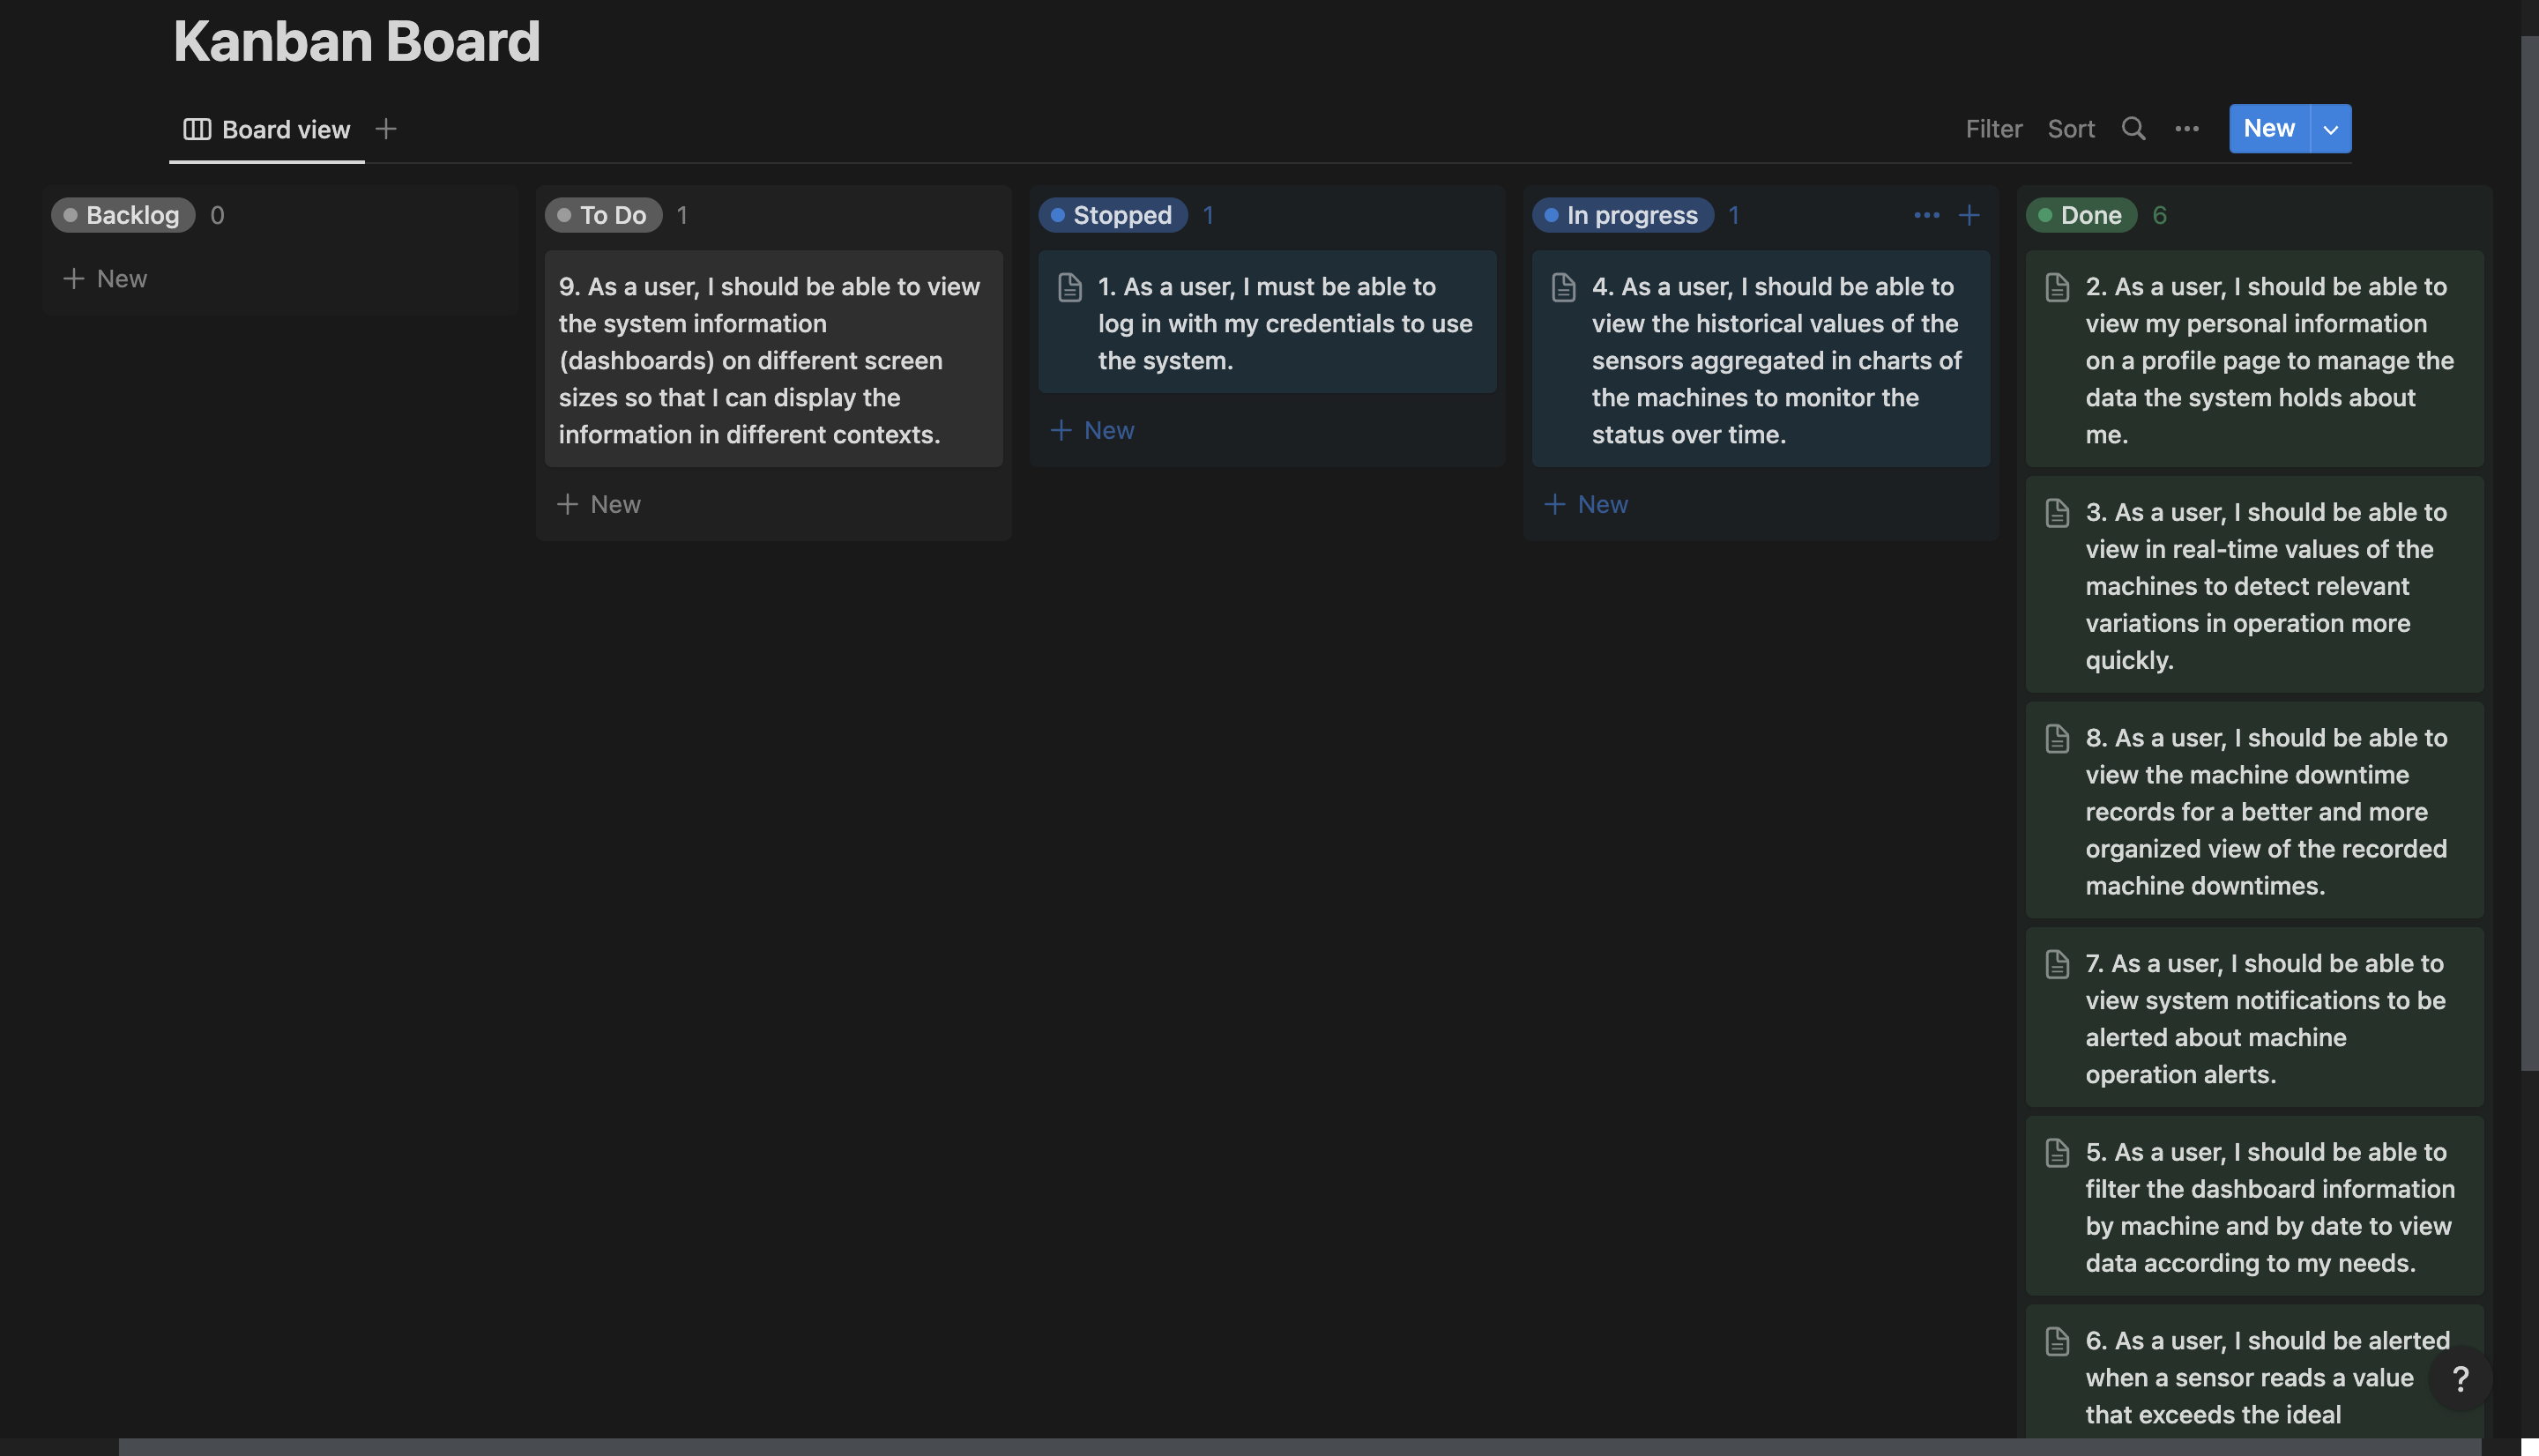
\includegraphics[width=\textwidth]{images/kanban_board}
	\caption{Board Kanban used to manager the tasks.}
	\label{fig:BoardKanban}
\end{figure}

A fim de definir melhor a implementação de cada história de usuário, cada card no board Kanban foi detalhado com uma descrição que inclui regras de negócio relevantes, referências a requisitos funcionais e não funcionais, critérios de aceitação e sub-tarefas. Antes que uma história de usuário possa ser movida para a coluna "In Progress", é essencial que esses campos sejam avaliados para assegurar um entendimento do escopo da tarefa. Os critérios de aceitação desempenham um papel importante na verificação de que uma história atende a todas as exigências estabelecidas antes de ser marcada como concluída.

Para ilustrar este processo, é detalhado a história de usuário número 1.

\textbf{1. As a user, I must be able to log in with my credentials to use the system.}
\begin{itemize}
    \item \textbf{Descrição:} Para garantir a segurança e a personalização da experiência do usuário, o sistema deve possuir uma funcionalidade de autenticação. O usuário deve inserir suas credenciais - geralmente um nome de usuário ou endereço de e-mail e uma senha - para acessar sua conta e as funcionalidades associadas a ela.
    \item \textbf{Regras de Negócio Relevantes:} 
        \begin{itemize}
            \item Os usuários não podem acessar o sistema sem autenticação.
            \item As tentativas de entrar no sistema devem ficar armazenadas no banco de dados.
            \item As senhas devem ser armazenadas de forma segura, utilizando técnicas como hashing.
        \end{itemize}

    \item \textbf{Referências a Requisitos:}
        \begin{itemize}
            \item \textbf{Funcionais:} FR1
            \item \textbf{Não Funcionais:} NFR2, NFR3, NFR6, NFR9 
        \end{itemize}

    \item \textbf{Critérios de Aceitação:}
        \begin{itemize}
            \item O sistema deve apresentar uma tela de login clara e intuitiva.
            \item Após inserir as credenciais corretamente, o usuário deve ser redirecionado para a página inicial do sistema (/dashboard).
            \item Se as credenciais estiverem incorretas, o usuário deve receber uma mensagem de erro clara.
        \end{itemize}

        \item \textbf{Sub-tarefas:}
            \begin{itemize}
                \item Desenhar a interface da tela de login.
                \item Construção da interface de login no repositório.
                \item Implementar a lógica de criação de usuário com hash de senha.
                \item Implementar a lógica de autenticação no backend com \gls{JWT} Token.
                \item Testar a segurança e eficácia da funcionalidade de login.
                \item Testar se a \gls{API} está retornando os códigos \gls{HTTP} corretamente.
            \end{itemize}

\end{itemize}



\subsection{Documentação do projeto}\label{sec:documentation}
%TODO ver se acho algo falando do notion como ferramenta de documentação - verificar se a referencia anterior ja não fala algo sobre
A documentação do projeto foi feita na ferramenta Notion. A escolha para este projeto foi fundamentada pois o Notion se destaca por sua flexibilidade, permitindo uma configuração adaptável dos texto para atender a vários tipos de necessidades. A interface intuitiva torna a inserção e atualização de informações um processo simples, que pode ser executado por ser uma plataforma acessível na internet por qualquer navegador.

Dessa forma, a documentação foi elaborada adotando uma abordagem estruturada para garantir que todas as características e funcionalidades fossem devidamente catalogadas. A base dessa documentação é uma tabela, onde cada entrada corresponde a uma funcionalidade ou a uma específica parte do sistema, sendo denominada de acordo com o nome da característica em questão.

Cada item da tabela se expande em uma página independente, com detalhes descritivos. Esta organização permite o entendimento em cada aspecto do sistema, pois foi sendo construído à medida que o sistema era desenvolvido, refletindo assim as adições e mudanças mais recentes.

Para facilitar a navegação e busca por informações específicas, foi incorporado uma coluna de tags na tabela. Estas tags servem para categorizar as funcionalidades, e também um mecanismo eficiente de busca, permitindo que os usuários identifiquem rapidamente os aspectos relevantes do sistema.

Além disso, o design interno de cada página é fundamentado na estrutura do markdown, explicado em \cite{markdownguide}, para assegurar que o conteúdo da documentação seja apresentado de forma clara, estruturada e esteticamente agradável, facilitando a compreensão e a absorção das informações por parte do leitor.

\subsection{Configuração dos repositórios}
A escolha da plataforma para gerenciamento dos repositórios do projeto foi o GitHub \cite{github}, uma das mais renomadas e amplamente adotadas plataformas de controle de versão baseada em Git disponíveis atualmente. A decisão de utilizar o GitHub foi pautada em alguns fatores. Primeiramente, a plataforma oferece uma interface intuitiva e um conjunto robusto de ferramentas que facilitam o acompanhamento do progresso do código, bem como a colaboração entre diferentes membros da equipe. Além disso, o GitHub é amplamente reconhecido por sua comunidade ativa, o que se traduz em uma vasta gama de recursos, tutoriais e suporte disponível, essencial para resolver possíveis dúvidas e desafios. Ademais, a integração com outras ferramentas e plataformas é facilmente realizável caso fosse necessário, permitindo um fluxo de trabalho contínuo e otimizado. Por fim, o compromisso do GitHub com a segurança, garantindo a integridade do código e dos dados do projeto, reforçou nossa decisão em adotá-lo como a solução de controle de versão para o projeto desenvolvido. 

Nesse contexto, os repositórios criados para esse projeto foram \texttt{backend}, que armazena o código referente a \gls{API} do sistema, outro chamado \texttt{frontend}, que armazena o código do dashboard que é exibido na web, e outro chamado \texttt{iot\_sensors\_data\_aggregation}, responsável por armazenar o código que realiza a agregação dos dados recebidos pelos sensores, o Modulo de Processamento dos Dados.


\subsection{Reuniões periódicas}
O desenvolvimento do projeto foi acompanhado por reuniões para garantir seu alinhamento com os objetivos do projeto. Reuniões semanais com o professor orientador foram estabelecidas, garantindo uma constante revisão, momento para tirar dúvidas, e realizar o detalhamento de atividades. Estes encontros proporcionaram um feedback contínuo, possibilitando a correção de trajetória e o foco no progresso desejado para o projeto. Paralelamente, reuniões mensais foram conduzidas com a empresa interessada, para apresentar o que estava sendo construído, pegar feedbacks, orientações sobre funcionalidades desejadas, e também entender melhor como funciona a empresa e suas necessidades.

Esses encontros desempenharam um papel fundamental na integração entre a pesquisa acadêmica e as necessidades práticas da indústria, buscando que as soluções desenvolvidas se mantivessem pertinentes e aplicáveis ao contexto empresarial. Este sistema de supervisão foi crucial para manter o projeto em seu curso, balanceando as necessidades acadêmicas com a aplicabilidade industrial dentro do contexto da empresa.


\section[Tecnologias]{Tecnologias}
A seleção de tecnologias foi realizada para atender a requisitos específicos de escalabilidade e sustentabilidade a longo prazo. Dado que o sistema é primariamente voltado para armazenamento e gestão de dados, foi antecipada sua utilização como referência para futuros projetos de características similares, por isso, a ênfase recaiu sobre tecnologias modernas, amplamente reconhecidas e com robusto suporte na comunidade de desenvolvimento.

Nesse contexto, o MongoDB foi escolhido como nossa solução de banco de dados não relacional, devido à sua flexibilidade e performance. Python foi adotado como linguagem para o backend, devido à sua versatilidade e ampla biblioteca. O framework FastAPI, por sua vez, foi empregado para a elaboração da \gls{API}, graças à sua eficiência e facilidade de integração. No âmbito do frontend, a linguagem JavaScript foi complementada pelo framework NextJs, reconhecido por sua otimização e recursos avançados. Para garantir uma integração fluida e modulada dos componentes do sistema, foi utilizado ao uso de containers Docker, enquanto o gerenciamento eficiente do servidor web foi assegurado pelo NGINX.

\subsection{MongoDB}
2-
Ao selecionar uma plataforma de banco de dados, optou-se pelo MongoDB \cite{mongodbDocs}, um sistema de banco de dados não relacional projetado para adaptar-se com flexibilidade às mudanças no formato dos dados que são armazenados. O MongoDB proporciona facilidade na manipulação do data lake em variados contextos. Sua documentação meticulosamente estruturada, aliada à vasta gama de conteúdo disponível online, provou ser inestimável para a aquisição de conhecimento.

Distintivamente, o MongoDB apresenta vantagens como a capacidade de suportar consultas distribuídas e paralelas, otimizando o processamento de requisições intrincadas em cenários com densidade significativa de dados. Adicionalmente, sua compatibilidade com uma ampla variedade de ferramentas de análise de dados estabelece um precedente promissor para evoluções futuras do projeto.

\subsection{Python}
%TODO colocar referencia para estudos que mostram a eficiência do python 
No desenvolvimento do backend, optou-se pela utilização da linguagem Python \cite{pythonOfficialDocs}, amplamente reconhecida por sua versatilidade, legibilidade e adaptabilidade em diversos contextos de aplicação. Python, sendo uma das linguagens mais populares e amplamente aceitas no mundo acadêmico e industrial, apresenta uma vasta biblioteca padrão e suporte comunitário robusto. A rica gama de materiais educativos, que abrange desde tutoriais detalhados até extensos fóruns de discussão, foi essencial para o aprendizado.

A sintaxe intuitiva de Python favorece a rápida prototipagem e desenvolvimento, ao passo que a ampla gama de frameworks e bibliotecas disponíveis potencializa sua aplicação em diversos aspectos, desde análise de dados até desenvolvimento web. Essas características intrínsecas, somadas à flexibilidade e eficiência da linguagem, consolidam a decisão de adotar Python como a linguagem central para o backend neste projeto de mestrado.


\subsection{FastAPI}
Na etapa de implementação do backend, decidiu-se empregar a linguagem Python, aliada ao framework FastAPI \cite{fastapiDocs}. Esta escolha foi motivada, em grande parte, pela eficácia e elevado desempenho oferecido pelo FastAPI. Este framework se destaca por incorporar a biblioteca \gls{ASGI}, uma interface que otimiza a gestão de solicitações, ao aproveitar ao máximo a execução assíncrona, garantindo respostas mais ágeis e precisas. Uma característica importante do FastAPI é sua documentação abrangente e bem elaborada, que ser como uma ferramenta fundamental ao processo de aprendizado e desenvolvimento.

\subsection{NextJs}
Para a arquitetura do frontend, optou-se pelo uso do Next.js \cite{nextjsDocs}, um framework que aprimora significativamente a interação com a biblioteca React \cite{reactDocs} do JavaScript, tal como enfatizado na própria documentação oficial do React. O suporte comunitário é uma de suas principais características, sendo amplamente complementado por uma oferta de materiais educativos disponíveis na internet - desde tutoriais a artigos de blog e vídeos instrucionais - os quais contribuíram de maneira essencial para o processo de aprendizado.

No escopo desse projeto, paralelamente ao Next.js, incorporou-se o TypeScript \cite{typescriptLang}, que por sua natureza de tipagem estática, proporciona uma manutenção do código mais intuitiva, incrementando sua legibilidade, simplificando sua compreensão e gerenciamento.

A coerência entre Next.js e TypeScript estabelece um ambiente de desenvolvimento altamente eficaz. Enquanto o Next.js promove uma experiência de desenvolvimento mais fluída e de alto desempenho, o TypeScript fortalece a segurança e a produtividade, graças à sua tipagem rigorosa. Estes fatores justificam a escolha da combinação de Next.js e TypeScript para a concretização deste projeto.

Além do Next.js e TypeScript, o Material UI 5 \cite{muiDocs} foi integrado ao projeto como biblioteca de design de interface do usuário. Este conjunto de componentes React, baseado no padrão de design Material Design da Google \cite{m3Docs}, oferece uma ampla gama de elementos de interface já estilizados e de fácil implementação. Além da economia de tempo no desenvolvimento de componentes desde o início, a biblioteca proporciona uma experiência de usuário coesa e moderna. O uso do Material UI 5 também contribui para a padronização do design em todo o projeto, assegurando uma experiência de usuário mais intuitiva e agradável. Portanto, a adição deste recurso complementa eficazmente as capacidades já robustas oferecidas pela combinação de Next.js e TypeScript, tornando o ambiente de desenvolvimento ainda mais rico e produtivo.

\subsection{Docker}
%TODO colocar referencia para artigo que mostra a eficiência do docker
Para a orquestração e gerenciamento do ambiente de desenvolvimento e produção, adotou-se o Docker \cite{dockerDocs} como ferramenta de containerização. O Docker, amplamente reconhecido no universo de desenvolvimento de software, possibilita encapsular aplicações e suas dependências em containers, garantindo uniformidade, reprodutibilidade e isolamento entre os ambientes. Esta abordagem simplifica significativamente os processos de integração, teste e implantação, uma vez que os containers podem ser movidos de forma transparente entre diferentes ambientes e plataformas.

A ampla documentação disponível, juntamente com uma comunidade ativa, proporcionou um entendimento claro e facilitou a adoção desta tecnologia. Além disso, a flexibilidade e eficiência proporcionadas pelo Docker, ao minimizar os conflitos de dependências e garantir que a aplicação funcione consistentemente em diversos contextos, foram fatores decisivos para sua escolha neste projeto.

\subsection{NGINX}
Para a parte de gestão das solicitações web, adotou-se o NGINX \cite{nginxDocs} como servidor web. O NGINX é reconhecido por sua alta performance, confiabilidade e flexibilidade, sendo uma escolha adequada em ambientes de produção que demandam baixa latência, tratamento eficiente de um grande número de conexões simultâneas, e com capacidade de servir conteúdo estático de maneira extremamente rápida. Essas características tornam-no particularmente adequado para sistemas que visam escalabilidade e robustez. 

A vasta documentação e os extensos recursos da comunidade foram essenciais para aprofundar o entendimento e aplicar as melhores práticas no contexto do projeto. Ao se considerar a necessidade de uma entrega consistente e otimizada do conteúdo ao usuário final, bem como uma configuração segura e eficaz do proxy, o NGINX se mostrou como a escolha preeminente para esta dissertação de mestrado.

\cleardoublepage
\chapter{Arquitetura do sistema}\label{cap:development}

In this chapter, you should describe the implementation, highlighting the most important aspects, the difficulties and the technical solutions that were followed. In particular, if code from others was used (available as open-source), should be easily identified.

\section[Diagrama do sistema]{Diagrama do sistema}
texto e a imagem....

\section[Princípios do SOLID]{Princípios do SOLID}
Topicos explicando cada uma das letras do SOLID e relacionando com exemplos concretos do sistema


\section[Arquitetura do backend]{Arquitetura backend}

\subsection*{API}
- Camada de recebimento das requisições
- Regras de negocio e modelos do sistema
- Camada de infraestrutura

\subsection*{Python Scripts}


\section[Arquitetura do frontend]{Arquitetura do frontend}
- Next JS e estrutura pre definida de pastas para as paginas do sistema
- Componentes e layouts
- Context API e seu uso
- Acesso a camada externa (API)

\section{Containers}
\cleardoublepage
\chapter{Implementação}\label{cap:implementation}

Após o capítulo onde a arquitetura do software foi detalhada, este capítulo é focado em explicar como tal arquitetura foi implementada, pois enquanto o primeiro descreve a estrutura e a organização, este foca nas ações técnicas adotadas para fazer essa estrutura funcionar.

Para uma análise mais estruturada e detalhada, este capítulo foi dividido em seções específicas para cada componente do sistema. São elas:

\begin{itemize}
    \item \textbf{Implementação do banco de dados}: Esta seção abordará os detalhes técnicos do design do banco de dados, esquemas adotados e como as informações são armazenadas e recuperadas.
    
    \item \textbf{Implementação do módulo de recebimento de dados}: Esta seção detalhará como os dados são recebidos, validados e processados antes de serem armazenados e disponibilizados para os usuários.
    
    \item \textbf{Implementação da API}: Aqui, a estrutura da API será discutida, passando pelos endpoints fornecidos, a lógica por trás de cada um e as camadas utilizadas.
    
    
    
    \item \textbf{Implementação do módulo de processamento de dados}: É abordado o tratamento dos dados recebidos pelos sensores, e como é feito a analise estatística que gera as informações apresentadas nos gráficos.
    
    \item \textbf{Implementação do frontend}: Por fim, a interface com o usuário será discutida, explicando como os dados são estruturados apresentados e apresentados em tela.
\end{itemize}

%TODO - Itens de implementação para adicionar;
% - Classe Singleton -
% - Classe ThreadManager -
% - Classe Datatype -
% - MetadataRepository -
% - iot_collection_parser.py - 
% - Pydantic - 
% - Envio de notificações via web socket - 



\section[Implementação do banco de dados]{Implementação do banco de dados}


\subsection[Organização do banco de dados]{Organização do banco de dados}

Dentro da implementação do sistema, o MongoDB foi usado para armazenar todas as informações do sistema. Este banco de dados, orientado a documentos, permitiu uma organização flexível dos dados, facilitando o armazenamento de diferentes dados que podem ser recebidos pelo modulo de recebimento de dados, e facilitando a criação de camadas de processamento. A estruturação dos bancos de dados e suas respectivas coleções foi pensada para facilitar tanto a inserção quanto a consulta de informações.

Em relação à organização dos dados, os seguintes bancos de dados foram criados:

\begin{itemize}
    \item \textbf{Users}: Armazena informações referentes aos usuários. Possui coleções que registram tentativas de login, detalhes pessoais dos usuários e tokens associados a eles.
    
    \item \textbf{Notification}: Destinado às notificações do sistema. Atualmente, este banco contém apenas notificações associadas aos alertas das máquinas, gerados pelos dados recebidos dos sensores junto com os parâmetros armazenados.
    
    \item \textbf{Downtime}: Armazena duas coleções, uma com os dados lidos das planilhas de parada das máquinas, e outro com esses dados tratados. Esse banco de dados com essas coleções são apenas para simular como ficaria os dados de parada das maquinas, caso eles fosses inseridos no sistema.
    
    \item \textbf{Raw Data}: Este banco é dedicado ao armazenamento de dados brutos oriundos de diferentes sensores. Cada tipo de sensor, como os sensores de pressão, tem sua própria coleção, garantindo um agrupamento das informações que facilita a análise.
    
    \item \textbf{Processed Data}: Como o próprio nome sugere, armazena dados que já passaram por uma etapa de processamento. Assim, dados interpretados de diferentes sensores são separados em coleções específicas, como os de pressão em uma e os de voltagem em outra.
    
    \item \textbf{Metadados}: Dedicado à armazenagem de metadados do sistema. Até o momento, a única coleção presente é a "AlertParameter", que reúne parâmetros utilizados para gerar alertas associados a cada sensor.
\end{itemize}

Com esta estruturação, busca-se não apenas organizar de forma lógica os dados, mas também otimizar operações de consulta e garantir uma expansão simplificada à medida que novas necessidades de armazenamento emergem no sistema.


\subsection[Acesso ao banco de dados]{Acesso ao banco de dados}

%TODO referencia para o motor
No processo de implementação do sistema, para estabelecer uma conexão eficiente com o banco de dados foi utilizado a biblioteca \texttt{motor} foi adotada como mecanismo.

No centro da estratégia de conexão está uma classe base, denominada \texttt{BaseDB}, que tem a responsabilidade não apenas de estabelecer a conexão com o MongoDB, mas também de definir uma série de operações básicas para a manipulação dos dados armazenados. A estrutura dessa classe é apresentada a seguir:

\begin{verbatim}
import motor
class BaseDB:
    def __init__(self):
        self.client = motor.motor_tornado.MotorClient(url, port)
\end{verbatim}

Algumas das operações fundamentais implementadas por \texttt{BaseDB} incluem:

\begin{itemize}
    \item \texttt{insert\_one}: Recebe como parâmetros o \textit{database} e a \textit{collection} correspondentes em formato de texto, e a \textit{data} a ser inserida. Insere um documento na coleção especificada.
    
    \item \texttt{insert\_many}: Recebe como parâmetros o \textit{database} e a \textit{collection} correspondentes em formato de texto, e a \textit{data} contendo vários documentos a serem inseridos. Insere vários documentos na coleção especificada.
    
    \item \texttt{read\_data\_with\_pagination}: Recebe como parâmetros o \textit{database}, a \textit{collection}, a \textit{query}, o \textit{page\_number}, o \textit{limit}, o \textit{sort\_descending\_field} e a \textit{projection}. Recupera dados com paginação, permitindo uma leitura mais organizada.
    
    \item \texttt{read\_data\_with\_limit}: Recebe como parâmetros o \textit{database}, a \textit{collection}, a \textit{query} e o \textit{limit}. Lê dados com um limite predefinido de documentos retornados.
    
    \item \texttt{read\_data}: Recebe como parâmetros o \textit{database}, a \textit{collection} e a \textit{query}. Realiza uma leitura simples de dados baseada em uma query.
    
    \item \texttt{get\_distinct\_property}: Recebe como parâmetros o \textit{database}, a \textit{collection} e a \textit{property}. Obtém propriedades distintas de uma coleção, verificando todos os documentos presentes.
    
    \item \texttt{list\_collections\_by\_db}: Recebe como parâmetro o \textit{database}. Lista todas as coleções presentes em um banco de dados específico.
    
    \item \texttt{add\_item\_into\_lists\_by\_filter}: Recebe como parâmetros o \textit{database}, a \textit{collection}, o \textit{filter}, as \textit{list\_properties} e a \textit{new\_data}. Adiciona um item em listas específicas baseado em um filtro.
    
    \item \texttt{update\_item}: Recebe como parâmetros o \textit{database}, a \textit{collection}, a \textit{data} a ser atualizada e o \textit{filter}. Atualiza um documento específico.
    
    \item \texttt{update\_many\_items}: Recebe como parâmetros o \textit{database}, a \textit{collection}, a \textit{data} a ser atualizada e o \textit{filter}. Atualiza vários documentos que atendam a um filtro.
    
    \item \texttt{count\_documents}: Recebe como parâmetros o \textit{database}, a \textit{collection} e a \textit{query}. Conta o número de documentos em uma coleção que atendem a uma consulta.
    
    \item \texttt{get\_data\_between\_dates}: Recebe como parâmetros o \textit{database}, a \textit{collection} e a \textit{query}. Recupera dados entre duas datas específicas.
\end{itemize}


Com a base de acesso estabelecida, outras classes foram desenvolvidas, herdados de \texttt{BaseDB}, para atender contextos específicos do sistema. Essas classes seguem o padrão singleton, o que garante que apenas uma instância da conexão seja criada para um contexto específico, otimizando a gestão dos recursos. Um exemplo é a classe \texttt{MongoDBIOT} destinada ao módulo de recebimento de dados:

\begin{verbatim}
class MongoDBIOT(BaseDB, metaclass=Singleton):
    def __init__(self):
        super().__init__()
\end{verbatim}

Classes semelhantes, seguindo o mesmo formato, foram criadas para outros contextos, como o acesso ao banco de dados pela API, garantindo uma estrutura organizada e eficiente de conexão e manipulação dos dados.

\section[Implementação do modulo de recebimento de dados]{Implementação do modulo de recebimento de dados}\label{sec:Implementação do modulo de recebimento de dados}

No processo de implementação do sistema, uma das etapas essenciais foi o desenvolvimento de um módulo destinado ao recebimento de dados provenientes dos sensores IoT. Este recebimento é realizado por meio de uma conexão multicast, uma abordagem eficiente para lidar com a transmissão de mensagens a vários destinatários simultaneamente.

Esse modulo é responsável por estabelecer a conexão multicast para receber os dados, realizar a conversão dos dados recebidos de acordo com o protocolo pré definido, disponibilizar os dados para serem mostrados em tempo real para os usuários conectados, verificar se gera algum tipo de alerta (e se gerar, notificar os usuários sobre isso com a criação de uma notificação), e salvar as informações geradas no banco de dados.

\subsection[Conexão e recebimento dos dados]{Conexão e recebimento dos dados}\label{subsec:Conexão e recebimento dos dados}

A classe \texttt{SensorConnection} tem como principal responsabilidade criar um socket, manter-se conectada para receber mensagens e interpreta-las. A estrutura e o funcionamento desta classe são detalhados a seguir.

A classe \texttt{SensorConnection} é iniciada com a criação de um socket IPv4 e UDP:

\begin{verbatim}
class SensorConnection:
    def __init__(self):
        self.sock = socket.socket(socket.AF_INET, socket.SOCK_DGRAM)
\end{verbatim}

Para garantir que o sistema esteja constantemente ouvindo mensagens multicast dos sensores, o método \texttt{listen\_multicast\_messages} foi definido dentro dessa classe. Ele invoca a criação da conexão e inicia o processo de leitura de mensagens, gerenciando ainda possíveis desconexões e reestabelecendo a ligação quando necessário:

\begin{verbatim}
    async def listen_multicast_messages(self, save_data_func):
        self.__create_connection()
        while True:
            await self.__start_read_messages(save_data_func)
            self.sock.close()
            time.sleep(1)
            self.__reconnect()
\end{verbatim}

A função \texttt{\_\_create\_connection} tem o papel de estabelecer e configurar a conexão inicial com o grupo multicast, e dentro do loop infinito é inciado o recebimento das mensagens com o método \texttt{\_\_start\_read\_messages}. Quando esse método é finalizado a conexão socket é fechada, e em seguida reconectada para depois voltar a fazer a leitura das mensagens. A chamada da função \texttt{time.sleep(1)} é utilizada para ter um pequeno intervalo entre uma chamada e outra caso e não realizar uma quantidade muito grande de chamadas caso esteja ocorrendo algum tipo de problema.

A seguir, cada uma das funções chamadas dentro desse método e detalhado.


\subsubsection[Método create connection]{Método create connection}

\begin{verbatim}
    def __create_connection(self):
        self.sock.setsockopt(socket.SOL_SOCKET, socket.SO_REUSEADDR, 1)

        server_address = ('', SENSOR_MULTICAST_PORT)
        self.sock.bind(server_address)

        multicast_group = SENSOR_MULTICAST
        group = socket.inet_aton(multicast_group)
        mreq = struct.pack('4sL', group, socket.INADDR_ANY)
        self.sock.setsockopt(socket.IPPROTO_IP, socket.IP_ADD_MEMBERSHIP, mreq)
\end{verbatim}

Inicialmente, o socket é configurado para permitir várias conexões em um único endereço. A opção \texttt{SO\_REUSEADDR} é definida com o valor 1, permitindo que mais de um socket se ligue a um mesmo endereço, o que é especialmente útil em contextos de conexões multicast:

\begin{verbatim}
    self.sock.setsockopt(socket.SOL_SOCKET, socket.SO_REUSEADDR, 1)
\end{verbatim}

Após isso, o socket é vinculado a um endereço e porta multicast específicos. É importante ressaltar que o primeiro argumento na definição do endereço do servidor é deixado vazio. Esta abordagem garante que o sistema esteja conectando-se com todas as interfaces de rede disponíveis, proporcionando uma ampla cobertura de conexão:

\begin{verbatim}
    server_address = ('', SENSOR_MULTICAST_PORT)
    self.sock.bind(server_address)
\end{verbatim}

Por fim, para se juntar efetivamente ao grupo multicast, algumas etapas são realizadas. O endereço IP multicast é primeiramente convertido para o formato binário com a chamada de \texttt{socket.inet\_aton}. Em seguida, este endereço e o endereço local (representado por \texttt{socket.INADDR\_ANY}) são empacotados em uma estrutura de dados por \texttt{struct.pack}. Esta estrutura é usado para especificar ao socket que ele deve se juntar a um grupo multicast em \texttt{self.sock.setsockopt}. A opção \texttt{IP\_ADD\_MEMBERSHIP} é definida e a estrutura previamente criada é passada como argumento, concluindo a conexão com o grupo multicast:

\begin{verbatim}
    multicast_group = SENSOR_MULTICAST
    group = socket.inet_aton(multicast_group)
    mreq = struct.pack('4sL', group, socket.INADDR_ANY)
    self.sock.setsockopt(socket.IPPROTO_IP, socket.IP_ADD_MEMBERSHIP, mreq)
\end{verbatim}

Essas operações garantem que o socket esteja configurado e conectado ao grupo multicast, pronto para receber mensagens de múltiplas fontes simultaneamente.


\subsubsection[Método reconnect]{Método reconnect}
\begin{verbatim}
def __reconnect(self):
    try:
        self.sock = socket.socket(socket.AF_INET, socket.SOCK_DGRAM)
        self.__create_connection()
    except Exception as e:
        print(f"Error to reconnect: {e}")
\end{verbatim}

Em situações em que a conexão com os sensores é interrompida, o método \texttt{\_\_reconnect} é chamado para tentar estabelecer novamente a conexão, criando uma nova instância do socket e chamando novamente a função \texttt{\_\_create\_connection}, detalhada anteriormente.

\subsubsection[Método start read messages]{Método start read messages}

\begin{verbatim}
async def __start_read_messages(self, save_data_func):
    while True:
        try:
            data, address = self.sock.recvfrom(1024)
            result = self.__parse_multicast_message(data)
            if not type(result) == str:
                await save_data_func(result)
        except Exception as e:
            print(f"Error: {e}")
            break
\end{verbatim}

Após as configurações realizads, as mensagens são continuamente lidas e processadas pela função \texttt{\_\_start\_read\_messages}. Durante este processo, cada mensagem é processada pelo método \texttt{\_\_parse\_multicast\_message}, e se estiver no formato correto, é passada para uma função que irá salvar e disponibilizar para API enviar por streaming para os usuários conectados.

Se ocorrer algum problema na execução desse método, ele é finalizado e volta para o \texttt{listen\_multicast\_messages}, onde o socket é fechado e uma nova conexão é estabelecida pelo método \texttt{\_\_reconnect}.


\subsubsection[Método parse multicast messages]{Método parse multicast messages}


\begin{verbatim}
def __parse_multicast_message(self, data):
        (machine_type_high, machine_number_low) = 
            self.__parse_bytes(data[:2])

        message_type = data[2]

        if message_type == 2:
            return "Request to publish..."

        (physical_quantity_high, sensor_number_low) = 
            self.__parse_bytes(data[3:5])
        
        (data_type_high, meaning_low) = 
            self.__parse_bytes(data[5:7])

        message_dict = {
            'Machine': {
                'Type': str(machine_type_high)+". "+MACHINE_TYPE[machine_type_high],
                'Number': machine_number_low
            },
            'Type': str(message_type)+". "+ MESSAGE_TYPE[message_type],
            'Sensor': {
                'PhysicalQuantity': PHYSICAL_QUANTITY[physical_quantity_high],
                'Number': sensor_number_low
            },
            'MeaningOfData': {
                'DataType': str(data_type_high)+". "+DATA_TYPE[data_type_high],
                'Meaning': str(meaning_low)+". "+DATA_MEANING[meaning_low]
            }
        }

        return message_dict
    \end{verbatim}



%TODO Colocar referencia para a arquitetura
Para interpretar e extrair informações da mensagem recebida do multicast, é crucial decodificar adequadamente a mensagem de acordo com o protocolo definido anteriormente. A implementação dessa decodificação é feita pelo método \texttt{\_\_parse\_multicast\_message}. A função auxiliar \texttt{\_\_parse\_bytes} é utilizada para essa tarefa, dada uma sequência de bytes, a função interpreta os bytes utilizando a ordem big-endian (onde os bytes mais significativos vêm primeiro).

\begin{verbatim}
def __parse_bytes(self, bytes):
    data = int.from_bytes(bytes, byteorder='big')
    high_data = (data >> 8) & 0xFF
    low_data = data & 0xFF

    return (high_data,low_data)
\end{verbatim}

Aqui, \texttt{data} contém o valor inteiro dos bytes fornecidos. O byte de ordem superior (High) é extraído deslocando o valor 8 bits para a direita e aplicando uma operação "END" (\&), e o byte de ordem inferior (Low) é simplesmente obtido aplicando a operação "END" com \texttt{0xFF}.

Com a capacidade de interpretar os bytes, a função principal \texttt{\_\_parse\_multicast\_message} pode começar a decodificação:

\begin{itemize}
    \item Primeiro, ela extrai o tipo de máquina e o número da máquina dos dois primeiros bytes da mensagem.
    
    \item O terceiro byte da mensagem é então interpretado como o tipo da mensagem. Se o tipo da mensagem for \texttt{2}, a função retornará diretamente uma solicitação para publicar.
    
    \item Os bytes 4 e 5 são interpretados como o ID do sensor, que contém a quantidade física sendo medida e o número do sensor.
    
    \item Os bytes 6 e 7 são usados para extrair o tipo de dados e seu significado.
\end{itemize}

A informação extraída é então organizada em um dicionário para representação clara e fácil acesso aos componentes individualmente:

\begin{verbatim}
message_dict = {
    'Machine': {
        ...
    },
    'Type': ...,
    'Sensor': {
        ...
    },
    'MeaningOfData': {
        ...
    }
}
\end{verbatim}

Esta estrutura permite uma representação clara e modular da mensagem decodificada, tornando fácil a integração e utilização em outras partes do sistema. Sendo assim, o retorno do método \texttt{\_\_parse\_multicast\_message} é utilizado como resultado da interpretação da mensagem multicast, e enviado para função recebida como parâmetro, \texttt{save\_data\_func}.

\subsection[Verificação e disponibilização dos dados]{Verificação e disponibilização dos dados}
No processo de recebimento dos dados, após abrir a conexão e os dados, é necessário verificar se estão no formato correto, se gera algum alerta, inserir no banco de dados e disponibilizar para os usuários conectados no sistema.

A classe \texttt{IotSensorConnection}, que implementa a interface \texttt{IotSensorConnectionInterface}, desempenha um papel principal neste módulo. Na sua inicialização, é estabelecida uma ligação com o repositório através da variável \texttt{self.\_\_repository}. Além disso, é responsável pela conexão com o sensor é estabelecida por meio do \texttt{self.\_\_sensor\_connection}, explicada anteriormente na seção ~\ref{subsec:Conexão e recebimento dos dados}.

\begin{verbatim}
class IotSensorConnection(IotSensorConnectionInterface):
    def __init__(self, respository:SensorsRepository):
        self.__repository = respository
        self.__sensor_connection = SensorConnection()
    
    def start_connection(self):
        threadManager = ThreadManager()
        threadManager.start_async_thread(self.__start_connection)
    
    async def __start_connection(self):
        await self.__sensor_connection.
            listen_multicast_messages(self.__handle_iot_data)
\end{verbatim}

%TODO Referencia para o helper de threads
Ao iniciar a conexão, utilizando o método \texttt{start\_connection}, é criada uma nova thread por meio da classe \texttt{ThreadManager}. Esta thread invoca o método \texttt{listen\_multicast\_messages} da classe \texttt{SensorConnection} que foi detalhado na seção ~\ref{subsec:Conexão e recebimento dos dados}. É necessário criar uma nova thread pois como esse modulo está junto com a API, e é necessário que os doi processos funcionem ao mesmo tempo, uma nova thread foi necessária para o funcionamento em paralelo de ambos.

\subsubsection{Verificação do formato dos dados}

%TODO referencia para a seção de helper do Pydantic
Para lidar com os dados recebidos, o método \texttt{\_\_handle\_iot\_data} é passado como argumento para \texttt{listen\_multicast\_messages} (como o argumento save\_func na classe que existe na classe \texttt{SensorConnection}).

%TODO Alterar o value no parse
\begin{verbatim}
async def __handle_iot_data(self, sensor_data:dict):
    sensor_model = self.__parse_sensor_data_to_sensor_model(sensor_data)
    await self.__repository.update_current_sensor_value(
        sensor_value = sensor_model.value,
        machine = sensor_model.machine,
        date = sensor_model.date,
        sensor_type = sensor_model.type,
        sensor_number = sensor_model.sensor_number
    )

def __parse_sensor_data_to_sensor_model(self, sensor_data:dict):
    value = 1
    machine = str(sensor_data["Machine"]['Number']) 
        + sensor_data["Machine"]['Type']
    date = datetime.now()
    data_type = sensor_data["Sensor"]["PhysicalQuantity"]
    sensor_number = sensor_data["Sensor"]["Number"]
    return ConnectionModelToParse(
        date=date,
        machine=machine,
        sensor_number=sensor_number,
        type=data_type,
        value=value
    )
\end{verbatim}

%TODO REFERENCIA PARA O PYDANTIC
Este método tem a responsabilidade de receber os dados so sensor e converter para uma classe modelo, denominada \texttt{ConnectionModelToParse}, que utiliza o \texttt{Pydantic} para validar as informações. O uso do \texttt{Pydantic} é mostrado na seção ~\ref{sec:a}.

\begin{verbatim}
from datetime import datetime
class ConnectionModelToParse:
    def __init__(self,value:float,machine:str,
        date:datetime,type:Datatype,
        sensor_number:int):

        self.value = value
        self.machine = machine
        self.date = date
        self.type = type
        self.sensor_number = sensor_number
\end{verbatim}

Após essa transformação, os dados são encaminhados para o repositório. O método \texttt{update\_current\_sensor\_value} do repository é chamado para checar se o dado recebido gera algum tipo de alerta, salvar no banco de dados, atualizar os dados em memoria, e realizar as verificações de notificação.

\begin{verbatim}
class SensorsRepository:
    def __init__(self):
        self.database = MongoDBIOT()
        self.iot_notification_check = IotNotificationCheck()
        self.__sensor_value = SensorValue()

    async def update_current_sensor_value(self, sensor_type:Datatype,
        sensor_value:float, machine:str, date:datetime, 
        sensor_number:int):
        alert_type = await self.__get_alert_type(sensor_value, sensor_type)
        current_value = {"machine":machine,
            "value":sensor_value, "timestamp": date,
            "alert_type":alert_type.value,
            "sensor_number":sensor_number}
        result = await self.insert_value_into_database(current_value, 
            sensor_type)
        new_id = result.inserted_id
        iot_data = IotData(
            alert_type=current_value["alert_type"],
            machine=current_value["machine"],
            timestamp=current_value["timestamp"],
            value=current_value["value"],
            id=PyObjectId(new_id),
            datatype=sensor_type,
            sensor_number=sensor_number
        )
        
        self.__sensor_value.update_sensor_value_by_type(
            iot_data,sensor_type)
        
        await self.iot_notification_check.check_iot_notification(
            iot_data)
\end{verbatim}

\subsubsection{Verificação de alertas}

Dentro do método \texttt{update\_current\_sensor\_value}, primeiramente é verificado o tipo de alerta gerado com a o método  \texttt{\_\_get\_alert\_type}.
%TODO Referencia para o helper de metadados com a leitura do parametro de alerta em get_sensor_alert_value
Esse método realiza a leitura do parâmetro de acordo do com tipo do sensor dentro dos metadados do sistema, em que o acesso é explicado em ..., e com ele verifica o status de alerta. 

O stats de alerta, definido pela função  \texttt{get\_alert\_status}, retorna como \texttt{OK} caso o valor do sensor seja menor que 90\% do valor definido com parâmetro, retorna como \texttt{WARNING} caso esse valor esteja entre 90\% e 100\%, e retorna como \texttt{PROBLEM} caso o valor retornado pelo sensor seja maior que 100\% do valor definido como parâmetro

\begin{verbatim}
def get_alert_status(self,sensor_value:int,
    alert_parameter:int)->AlertTypes:

    parameter = ((sensor_value/alert_parameter)*100)
    if parameter < 90:
        return AlertTypes.OK
    if parameter >= 90 and parameter < 100:
        return AlertTypes.WARNING
    if parameter >= 100:
        return AlertTypes.PROBLEM

async def __get_alert_type(self, sensor_value:float,
    sensor_type:Datatype)->AlertTypes:
    alert_parameter = await MetadataRepository()
        .get_sensor_alert_value(sensor_type)
    alert_type = self.get_alert_status(sensor_value,alert_parameter)
    return alert_type
\end{verbatim}


\subsubsection{Registro no banco de dados}

Com a verificação dos alertas, todas as informações foram geradas, portanto já podem ser registradas no banco de dados. Para esse registro é usado o método \texttt{insert\_value\_into\_database}.

\begin{verbatim}
async def insert_value_into_database(self, value:BaseIotData, type:Datatype):
    try:
        collection = sensor_name_to_raw_data_collection(type)
        return await self.database.insert_one(IOT_DATABASE,collection,value)
    except Exception as ex:
        print(ex)
        raise ex
\end{verbatim}

Esse método utiliza da classe base do banco de dados com operações já definidas para realizar o registro. Dentro do método \texttt{update\_current\_sensor\_value} do repositório, o retorno é utilizado para manter o ID registrado em memoria, importante para criar o objeto \texttt{IotData}, que é enviado para os usuários conectados, via stream, no passo seguinte.

\begin{verbatim}
current_value = {"machine":machine,
    "value":sensor_value,
    "timestamp": date,
    "alert_type":alert_type.value,
    "sensor_number":sensor_number}
result = await self.insert_value_into_database(current_value, sensor_type)
new_id = result.inserted_id
iot_data = IotData(
    alert_type=current_value["alert_type"],
    machine=current_value["machine"],
    timestamp=current_value["timestamp"],
    value=current_value["value"],
    id=PyObjectId(new_id),
    datatype=sensor_type,
    sensor_number=sensor_number
)
\end{verbatim}

%TODO Referencia para a seção de helpers quando pega o nome da collection
Uma informação importante a se destacar, é que o nome da coleção utilizada pelo método \texttt{insert\_value\_into\_database} é definida de acordo com tipo de dado estabelecido, usando a função de ajuda \texttt{sensor\_name\_to\_raw\_data\_collection}, explicada anteriormente em ....

\subsubsection{Atualização dos dados em memoria}

Com o tipo de alerta definido e os dados registrados no banco de dados, é utilizado a classe \texttt{SensorValue} para atualizar as informações na memória. Esse processo é feito por meio da chamada \texttt{\_\_sensor\_value.update\_sensor\_value\_by\_type (iot\_data,sensor\_type)} no método \texttt{update\_current\_sensor\_value} do repository.


A classe \texttt{SensorValue} é responsável por gerenciar e atualizar os valores em memória. Nota-se que a mesma utiliza o padrão de projeto \texttt{Singleton}, assegurando a existência de apenas uma instância desta classe durante todo o ciclo de vida da aplicação, garantindo que so existe uma instancia armazenando as informações dos sensores.

\begin{verbatim}
class SensorValue(metaclass=Singleton):
    def __init__(self) -> None:
        self.machine_list:list[MachineData] = []

    def update_sensor_value_by_type(self, new_value: IotData, data_type: Datatype):
        is_new_machine = True

        for machine in self.machine_list:
            if machine.name == new_value.machine:
                is_new_machine = False
                is_new_sensor = True

                for index, sensor in enumerate(machine.sensor_data):
                    if sensor.datatype == data_type:
                        machine.sensor_data[index] = new_value
                        is_new_sensor = False
                        break

                if is_new_sensor:
                    machine.sensor_data.append(new_value)
                    break

        if is_new_machine:
            new_machine = MachineData(name=new_value.machine,sensor_data=[new_value])
            self.machine_list.append(new_machine)
\end{verbatim}

No momento de sua inicialização, a classe \texttt{SensorValue} inicializa uma lista vazia, \texttt{machine\_list}, que será responsável por armazenar os valores dos sensores organizados por máquina.

A atualização acontece pelo método \texttt{update\_sensor\_value\_by\_type}. Este método atualiza o valor do sensor na memória de acordo com seu tipo (\texttt{data\_type}). O processo de atualização verifica primeiramente se a máquina associada ao sensor já existe na lista. Caso positivo, busca-se pelo sensor específico dentro dos dados da máquina e atualiza-se seu valor. Se o sensor não for encontrado, um novo é adicionado à lista de sensores da máquina correspondente.

Por outro lado, se a máquina não for encontrada na lista \texttt{machine\_list}, uma nova instância de \texttt{MachineData} é criada e adicionada à lista, contendo as informações da máquina e os dados do sensor recebido.

\begin{verbatim}
class MachineData(BaseModel):
    name:str = Field(...)
    sensor_data:list[IotData] = Field([])
\end{verbatim}

Dessa forma, o repositório envia as informações para esse método, e com a verificação adequada, é mantido os dados mais atualizados em memoria, e disponível para ser utilizado pela API, possibilitando o acesso em tempo real dos dados dos sensores.


\subsubsection{Verificação de notificação}
Com o tipo de alerta verificado, a informação salva no banco de dados e o objeto \texttt{IotData} montado, a última tarefa do método \texttt{update\_current\_sensor\_value} do repository é utilizar o singleton IotNotificationCheck para verificar as notificações em relação a operação das máquinas.

A classe \texttt{IotNotificationCheck} atua como um controlador de alertas para dados IoT. Ao receber dados IoT, ela verifica o estado do alerta e toma medidas apropriadas, seja adicionando ou removendo máquinas ou sensores da lista de alertas. Essa classe é essencial para monitorar e responder a eventos de alerta em tempo real, garantindo que os usuários associados sejam notificados de quaisquer anormalidades ou eventos importantes detectados pelos sensores IoT.

Por meio do método \texttt{check\_iot\_notification}, a classe verifica o tipo de alerta recebido pelo objeto IotData, se a máquina está em estado de alerta e se o sensor específico da máquina está em estado de alerta. Com base nessa verificação, o método toma uma das seguintes ações:

\begin{enumerate}
    \item Coloca uma nova máquina em estado de alerta.
    \item Coloca um novo sensor da máquina em estado de alerta.
    \item Remove um sensor da máquina do estado de alerta. Se a máquina tiver apenas um único sensor em estado de alerta, a maquina é removida do estado de alerta
\end{enumerate}


\begin{verbatim}
async def check_iot_notification(self, iot_data:IotData):
    is_alert_value = self.__is_alert_type_a_new_alert(
        iot_data.alert_type)
    machine_in_alert = self.__is_machine_in_alert_state(
        machine_name=iot_data.machine)
    machine_sensor_in_alert = self.__is_machine_sensor_in_alert_state(
        machine_in_alert,
        iot_data.datatype)

    is_machine_in_alert = machine_in_alert!=None

    if is_alert_value and is_machine_in_alert and (not machine_sensor_in_alert):
        await self.__put_new_machine_sensor_in_alert_state(
            machine_in_alert,
            iot_data.datatype)

    if is_alert_value and (not is_machine_in_alert):
        await self.__put_new_machine_in_alert_state(
            iot_data.machine,
            iot_data.datatype,
            iot_data.timestamp,
            iot_data.alert_type)

    if (not is_alert_value) and is_machine_in_alert and machine_sensor_in_alert:
        await self.__remove_machine_sensor_from_alert_state(
            machine_in_alert,
            iot_data.datatype,
            iot_data.timestamp)
\end{verbatim}

%TODO referencia para o datatype
O método \texttt{\_\_put\_new\_machine\_sensor\_in\_alert\_state} é um método assíncrono privado que tem a responsabilidade de adicionar um novo sensor ao estado de alerta para uma máquina específica. Ele recebe dois parâmetros: \texttt{machine\_in\_alert}, que é uma instância da classe \texttt{MachinesSensorAlert} representando a máquina em questão, e \texttt{sensor\_type}, que é uma instância do tipo \texttt{Datatype} representando o tipo de sensor que deve ser colocado em alerta.

\begin{verbatim}
class MachinesSensorAlert(BaseModel):
    id: PyObjectId = Field(default_factory=PyObjectId, alias="_id")
    machine:str = Field(...)
    sensors:list[str] = Field([])
    alert_type:str = Field(...)
    start_time:datetime = Field(...)
    sensors_historical:list[str] = Field([])
    is_in_alert:bool = Field(True)
    
    end_time:Optional[datetime|None] = Field(None)
    read_by:Optional[list[str]] = Field([])
\end{verbatim}

Importante destacar que dentro dessa instância que é mantida em memória, o atributo \texttt{read\_by} não é preenchido. Isso acontece pois esse atributo é usado para controlar os usuários que marcaram a notificação como lida, portanto é preenchida apenas no banco de dados. A implementação da parte de notificações que faz uso desse atributo pode ser lida na seção ....%TODO Referencia para a seção que mostra a implementação das notifcações


A primeira etapa realizada por este método é identificar a posição (ou índice) da máquina dentro da lista de alertas \texttt{machines\_alert} usando o método \texttt{index}. Uma vez obtido o índice, o tipo do sensor é adicionado à lista de sensores em estado de alerta da máquina, representada pelo atributo \texttt{sensors}. Além disso, este sensor também é adicionado ao histórico de sensores em estado de alerta da máquina, indicado pelo atributo \texttt{sensors\_historical}. Finalmente, a máquina atualizada (com o novo sensor adicionado às suas listas de alerta e histórico) é reinserida na lista principal \texttt{machines\_alert} na mesma posição identificada anteriormente.

Este método, garante que sempre que um novo sensor entra em estado de alerta para uma máquina que ja tinha um sensor em alerta, as informações relevantes são adequadamente atualizadas e mantidas em memória, permitindo um acompanhamento em tempo real das condições de alerta de todas as máquinas monitoradas.

\begin{verbatim}
async def __put_new_machine_sensor_in_alert_state(
        self,
        machine_in_alert: MachinesSensorAlert,
        sensor_type:Datatype):
    index = self.machines_alert.index(machine_in_alert)
    machine_in_alert.sensors.append(sensor_type.value)
    machine_in_alert.sensors_historical.append(sensor_type.value)
    self.machines_alert[index] = machine_in_alert
\end{verbatim}

Já o método \texttt{\_\_put\_new\_machine\_in\_alert\_state} é um método assíncrono privado cuja principal função é criar e registrar um novo estado de alerta para uma máquina específica. Este método é invocado quando uma máquina entra em estado de alerta pela primeira vez, o que significa que ainda não está presente na lista de alertas \texttt{machines\_alert} da classe.

%TODO referencia para o datatype
Recebe quatro parâmetros: \texttt{machine\_name}, que é uma string representando o nome da máquina; \texttt{sensor\_type}, que é uma instância do tipo \texttt{Datatype} denotando o tipo de sensor que disparou o alerta; \texttt{start\_time}, uma instância de \texttt{datetime} indicando o início do alerta; e \texttt{alert\_type}, que é uma string representando o tipo de alerta.

Inicialmente, o método cria uma nova instância da classe \texttt{MachinesSensorAlert}. Esta nova instância representa o estado de alerta da máquina. A instância é inicializada com o nome da máquina, o tipo de sensor que causou o alerta, uma marca temporal do início do alerta e o tipo de alerta. Além disso, a máquina é marcada como estando em estado de alerta através do atributo \texttt{is\_in\_alert}, que é definido como \texttt{True}.

Finalmente, o novo estado de alerta da máquina, representado pela instância \texttt{MachinesSensorAlert} recém-criada, é adicionado à lista \texttt{machines\_alert}.

\begin{verbatim}
async def __put_new_machine_in_alert_state(self,
    machine_name:str,
    sensor_type:Datatype,
    start_time:datetime,
    alert_type:str):

    new_machine_alert = MachinesSensorAlert(
        machine=machine_name,
        sensors=[sensor_type.value],
        sensors_historical=[sensor_type.value],
        is_in_alert=True,
        start_time=start_time,
        alert_type=alert_type)

    self.machines_alert.append(new_machine_alert)
\end{verbatim}


%TODO referencia para o datatype
O método \texttt{\_\_remove\_machine\_sensor\_from\_alert\_state} é uma função assíncrona privada projetada para remover um sensor específico do estado de alerta de uma máquina. Ele recebe três parâmetros: \texttt{machine\_in\_alert}, que é uma instância da classe \texttt{MachinesSensorAlert} representando a máquina em questão; \texttt{sensor\_to\_remove}, que é do tipo \texttt{Datatype} e identifica o sensor a ser removido; e \texttt{end\_time}, uma instância de \texttt{datetime} que indica o momento em que o sensor foi removido do estado de alerta. Dentro deste método, inicialmente, as posições do sensor e da máquina são identificadas nas listas apropriadas. O sensor é então removido da lista de sensores em estado de alerta da máquina. Se, após a remoção, a máquina não tiver mais sensores em estado de alerta, ela será removida do estado de alerta, pela chamada do método \texttt{\_\_remove\_machine\_from\_alert} caso contrário, apenas o estado do sensor é atualizado, pela chamada de outro método, \texttt{\_\_remove\_sensor\_from\_alert\_state}.

\begin{verbatim}
async def __remove_machine_sensor_from_alert_state(self,
    machine_in_alert: MachinesSensorAlert,
    sensor_to_remove:Datatype,
    end_time:datetime):
    index_of_machine = self.machines_alert.index(machine_in_alert)
    index_of_sensor = machine_in_alert.sensors.index(sensor_to_remove.value)
    
    machine_in_alert.sensors.pop(index_of_sensor)
    
    if len(machine_in_alert.sensors) == 0:
    await self.__remove_machine_from_alert(index_of_machine, end_time)
    else:
    await self.__remove_sensor_from_alert_state(index_of_machine,machine_in_alert)
    
\end{verbatim}

O método \texttt{\_\_remove\_machine\_from\_alert} é outra função assíncrona privada, que tem a responsabilidade de remover completamente uma máquina do estado de alerta. Aceita dois parâmetros: \texttt{index\_of\_machine}, o índice da máquina em questão na lista, e \texttt{end\_time}, o momento em que a máquina foi removida do alerta. Dentro deste método, a máquina é primeiro marcada como não estando em alerta e depois é removida da lista \texttt{machines\_alert}. A máquina é então armazenada no banco de dados com um registro de seu estado final e o horário de término. Finalmente, uma notificação é enviada através de um websocket para informar a interface do usuário sobre a mudança no estado da máquina. O detalhamento de como a notificação é enviada está explicada em X %TODO referencia aqui para as notificações

\begin{verbatim}
async def __remove_machine_from_alert(self,
    index_of_machine:int,
    end_time:datetime):
    machine_in_alert = self.machines_alert[index_of_machine]
    machine_in_alert.is_in_alert = False
    machineNotification = self.machines_alert.pop(index_of_machine)
    machineNotification.end_time = end_time
    await self.iot_database.insert_one(
    NOTIFICATION_DATABASE,
    IOT_MACHINE_ALERTS,
    machineNotification.to_bson())
    await self.websocket.send_notification(machineNotification)    
\end{verbatim}

O método \texttt{\_\_remove\_sensor\_from\_alert\_state} é uma função assíncrona simples que atualiza o estado do sensor de uma máquina em alerta na lista de máquinas em alerta. Recebe dois parâmetros: \texttt{index\_of\_machine}, que é o índice da máquina na lista \texttt{machines\_alert}, e \texttt{machine\_alert\_updated}, que é a instância atualizada da máquina em alerta. Essencialmente, este método substitui a máquina existente na lista pelo objeto atualizado fornecido como parâmetro pelo método \texttt{\_\_remove\_machine\_sensor\_from\_alert\_state}.

\begin{verbatim}
async def __remove_sensor_from_alert_state(self,
    index_of_machine:int,
    machine_alert_updated:MachinesSensorAlert):
    self.machines_alert[index_of_machine] = machine_alert_updated
\end{verbatim}



\section[Implementação do módulo de processamento de dados]{Implementação do módulo de processamento de dados}
%TODO Ref para o cap que explica a arquitetura dessa parte
Como explicado em X, o modulo de processamento de dados faz a leitura dos dados brutos do sistema, aplica faz o calculo do boxplot e armazena o resultado no banco de dados.

\subsection{Agendamento para execução periódica}
%TODO Referencia para a biblioteca schedule
O processamento dos dados precisa ocorrer periodicamente, no caso foi definido inicialmente uma vez por dia. Para executar a chamada da função de processamento uma vez ao dia foi utilizado a biblioteca schedule. Com essa biblioteca foi agendado para todo dia meia noite a execução da função da função de inicia a agregação dos dados. Um loop infinito foi criado para manter o código em execução, verificando se a função deve ser executada ou não.

\begin{verbatim}
import schedule
schedule.every().day.at("00:00").do(aggregation_init)
print(datetime.now(), flush=True)
while True:
    schedule.run_pending()
    time.sleep(1)
\end{verbatim}

\subsection{Identificando a origem dos dados}
Dentro desta estrutura, é necessário identificar as coleções corretas das quais os dados devem ser recuperados antes de realizar o processamento. Essa identificação começa pela função \texttt{get\_tuples\_with\_raw\_data\_collections\_and\_processed\_collections()}. Esta função, como o próprio nome sugere, está encarregada de recuperar tuplas relacionando as coleções de dados brutos com suas respectivas coleções processadas. Itera-se sobre todos os tipos de sensores, representados pelo enumerador \texttt{Datatype}, e para cada tipo de sensor, identificam-se as respectivas coleções de dados brutos e processados, resultando em uma lista de tuplas. 

Importante destacar que os nomes das coleções são recuperados pelas funções de ajuda, explicados em %TODO Referencia para função helper que gera nome das coleções...

\begin{verbatim}
def get_tuples_with_raw_data_collections_and_processed_collections():
    result:list[tuple] = []
    for sensor_type in Datatype:
        raw_collection = sensor_name_to_raw_data_collection(
        sensor_type)
        processed_collection = sensor_name_to_processed_collection(
        sensor_type)
        result.append((raw_collection,processed_collection))
    return result
\end{verbatim}

%TODO Sigla API
Para iniciar o processamento dos dados, a função \texttt{aggregation\_init()} foi desenvolvida. Ao ser chamada, essa função primeiramente obtém a lista de tuplas que relaciona as coleções de dados brutos com as processadas. Após recuperar esta lista, ela inicializa um loop assíncrono, cujo objetivo é executar uma função de agregação até sua conclusão. Esse design assíncrono é crucial para garantir que o processamento possa realizar chamadas de funções assíncronas, dado que esse modulo é separado da API.

\begin{verbatim}
def aggregation_init():
    tuples_list = 
    get_tuples_with_raw_data_collections_and_processed_collections()

    loop = asyncio.new_event_loop()
    loop.run_until_complete(aggregation(tuples_list))
    loop.close()
\end{verbatim}

Desta forma, a correta identificação da origem dos dados, juntamente com as funções explicadas, estabelece qual a origem dos dados que devem ser processados

\subsection{Iniciando a agregação}
Uma vez definida a origem dos dados por meio das coleções identificadas, a fase de agregação dos dados é iniciada. A função responsável por essa tarefa é a \texttt{aggregation()}, que aceita uma lista de tuplas representando as coleções de sensores.

\begin{verbatim}
async def aggregation(sensors_collection_list:list[tuple]):
    database = BaseDB()
    for collection_tuple in sensors_collection_list:
        (raw_data_collection, processed_data_collection) = collection_tuple
        machine_list = await database.read_machines_list(raw_data_collection)

        for machine in machine_list:
            await aggregate_data(database, raw_data_collection, processed_data_collection, machine)
\end{verbatim}

%TODO referencia para base DB
Dentro desta função, primeiramente, uma instância da base de dados é inicializada usando a classe \texttt{BaseDB()}. Em seguida, a função itera sobre cada tupla na lista fornecida. Para cada tupla, as coleções de dados brutos e processados são extraídas. Utilizando a coleção de dados brutos como referência, é feita uma leitura da lista de máquinas associadas a essa coleção por meio do método \texttt{read\_machines\_list()}.

\begin{verbatim}
async def read_machines_list(self, collection:str):
    try:
        temp_client = self.client
        return await temp_client[IOT_DATABASE][collection].distinct('machine')
    except Exception as ex:
        print(ex)
        raise ex
\end{verbatim}


Para cada máquina identificada, os dados são então agregados. A função \texttt{aggregate\_data()} é chamada, passando-se a base de dados, a coleção de dados brutos, a coleção de dados processados e a máquina específica em questão como argumentos. Esta função, por sua vez, é responsável por realizar a efetiva agregação dos dados da máquina, transformando dados brutos em dados processados que serão armazenados na respectiva coleção de dados processados.

\subsubsection{Busca dos dados a serem agregados}
Inicialmente, um \texttt{query} é gerado utilizando a função \texttt{get\_aggregation\_query()}, que usa as informações da coleção agregada e da máquina em questão. Com esta \texttt{query}, os dados brutos são então lidos da coleção de dados brutos usando o método \texttt{read\_raw\_data()}.

A função \texttt{get\_aggregation\_query()} é encarregada de gerar a \textit{query} que busca as informações a serem agregadas pelo modulo de processamento. O objetivo dela é que apenas os dados brutos ainda não processados sejam considerados para agregação, otimizando o processo e evitando reprocessamento desnecessário.

Esta função necessita de uma instância da base de dados, o nome da coleção onde os dados agregados são armazenados e a máquina específica para a qual a agregação é necessária.

\begin{verbatim}
async def get_aggregation_query(
    database:BaseDB,
    collection:str,
    machine:str)->dict:
    field_to_aggregate = "more_recent_register"
    more_recent_processed_data:BoxPlotData|None = 
    await database.read_more_recente_data(
        collection,
        machine,
        field_to_aggregate)
    
    if more_recent_processed_data is None:
        return __build_query_with_limit_of_data(machine) 
    else:
        return __build_query_with_range_of_data(
        more_recent_processed_data,
        machine,
        field_to_aggregate)
\end{verbatim}

Inicialmente, o campo \texttt{more\_recent\_register} é definido como o atributo a ser buscado. A função \texttt{read\_more\_recente\_data()} é então chamada para obter os dados processados mais recentes para a máquina e coleção em questão.

\begin{verbatim}
async def read_more_recente_data(self,
    collection:str,
    machine:str,
    date_time_field:str):
    try:
        temp_client = self.client
        cursor = temp_client[IOT_PROCESSED_DATA][collection].find({"machine":machine}).sort([(date_time_field,pymongo.DESCENDING)])
        result:list = await cursor.to_list(None)
        return result[0] if len(result)!= 0 else None
    except Exception as ex:
        print(ex)
        raise ex
\end{verbatim}

Se nenhum dado processado recente for encontrado, a \textit{query} é construída utilizando a função \texttt{\_\_build\_query\_with\_limit\_of\_data()}. Esta função simplesmente limita a quantidade de dados recuperados a \texttt{MAX\_VALUE\_BY\_PERIOD} e busca por registros que correspondam à máquina especificada.

\begin{verbatim}
def __build_query_with_limit_of_data(machine:str)->dict:
    return {
        "limit":MAX_VALUE_BY_PERIOD,
        "query":{"machine":machine}
    }
\end{verbatim}


No entanto, se dados processados recentes forem encontrados, a função a ser utilizada é a \texttt{\_\_build\_query\_with\_range\_of\_data()}. Esta função considera o registro processado mais recente e calcula um intervalo de tempo (\texttt{date\_limit\_to\_process\_data}) adicionando o período de agregação, definido por \texttt{AGGREGATION\_PERIOD\_IN\_HOURS}, à data desse registro mais recente. A \textit{query} gerada busca registros com \textit{timestamps} dentro desse intervalo de tempo e que correspondam à máquina especificada, com um limite máximo de 
registros definido por \texttt{MAX\_VALUE\_BY\_PERIOD}.

\begin{verbatim}
def __build_query_with_range_of_data(more_recent_processed_data:BoxPlotData,
machine:str,
field_to_aggregate:str)->dict:
    date_of_more_recent:datetime = 
    more_recent_processed_data[field_to_aggregate]

    date_limit_to_process_data = date_of_more_recent + 
    timedelta(hours = AGGREGATION_PERIOD_IN_HOURS)

    return {
        "query":{
            "timestamp": {
                "$gt": date_of_more_recent,
                "$lte": date_limit_to_process_data
            },
            "machine":machine
        },
        "limit":MAX_VALUE_BY_PERIOD
    }

\end{verbatim}

\subsubsection{Calculo do BoxPlot}
Com query montada, os dados são recuperados com a função \texttt{read\_raw\_data}.

\begin{verbatim}
async def read_raw_data(self, collection:str, query:dict):
    try:
        temp_client = self.client
        cursor = temp_client[IOT_DATABASE][collection].find(
            query["query"])
            .sort([("timestamp",pymongo.ASCENDING)])
            .limit(query["limit"])
        return await cursor.to_list(None)
    except Exception as ex:
        print(ex)
        raise ex
\end{verbatim}

A quantidade de dados recuperados é calculada e, se esta quantidade exceder um valor mínimo predefinido (\texttt{MINIMUM\_DATA\_TO\_AGGREGATE}), a agregação prossegue. Caso não seja atingindo a quantidade mínima, a função recursiva é finalizada, concluído o processamento dos dados daquela coleção.

Apos a busca da query, um objeto \texttt{logger} é inicializado para manter registros do processo de agregação.

%TODO referencia para trabalhos futuros com melhoria de logs
Nessa implementação o log é utilizado apenas para mostrar informações no console, mas uma implementação futura pode adicionar uma forma mais completa de logs.

\begin{verbatim}
class Logger(metaclass=Singleton):
    async def store_aggregation_log(self,box_plot_data:BoxPlotData, collection:str):
        print("+++++++++++++++++++++++++++++")
        print("Collection {}".format(collection))
        print("more_recent_register {}".format(box_plot_data.more_recent_register))
        print("median {}".format(box_plot_data.median))
        print("mean {}".format(box_plot_data.mean))
        print("q1 {}".format(box_plot_data.q1))
        print("q3 {}".format(box_plot_data.q3))
        print("lower_quartile {}".format(box_plot_data.lower_quartile))
        print("upper_quartile {}".format(box_plot_data.upper_quartile))
        print("mean_with_selection {}".format(box_plot_data.mean_with_selection))
        print("amount_of_data {}".format(box_plot_data.amount_of_data))
        print("+++++++++++++++++++++++++++++")

    async def not_aggregated_data(self, amount:int, collection:str):
        print("=============================")
        print("")
        print("Amount data not aggregated {} - {}".format(str(amount),collection))
        print("=============================")
\end{verbatim}

%TODO referencia para o pandas
Os dados brutos lidos do banco de dados são convertidos em um DataFrame do pandas (biblioteca da linguagem python utilizada para manipulação e dados), após o qual são calculados os dados agregados relevantes usando a função \texttt{calc\_box\_plot()}. Esta função retorna os dados em uma forma estruturada adequada para representações gráficas, como um box plot.

\begin{verbatim}
def calc_box_plot(df:pd.DataFrame, machine:str):
    values = df["value"]

    median = values.median()
    mean = values.mean()

    Q1 = values.quantile(.25)
    Q3 = values.quantile(.75)

    IIQ = Q3 - Q1

    lower_quartile = Q1 - 1.5 * IIQ
    upper_quartile = Q3 + 1.5 * IIQ
    
    selection = (df["value"]>=lower_quartile) & (df["value"]<=upper_quartile)

    values_selected = values[selection]
    
    mean_with_selection = values_selected.mean()

    df['timestamp'] = pd.to_datetime(df['timestamp'])
    date_of_more_recent:datetime|str = df['timestamp'].max()

    amount_of_data = df.shape[0]

    box_plot = BoxPlotData()

    box_plot.more_recent_register:datetime = date_of_more_recent

    box_plot.lower_quartile=lower_quartile
    box_plot.upper_quartile=upper_quartile
    box_plot.median=median
    box_plot.mean=mean
    box_plot.mean_with_selection=mean_with_selection
    box_plot.q1=Q1
    box_plot.q3=Q3
    box_plot.amount_of_data=amount_of_data
    box_plot.machine=machine

    return box_plot
\end{verbatim}


Nessa função, o dataframe recebido contém uma série de valores que será utilizada para calcular os componentes do Box Plot. Primeiro, são determinados os valores da mediana e da média dos dados. Os quartis Q1 (primeiro quartil) e Q3 (terceiro quartil) são calculados utilizando a função \texttt{quantile()}, da bilbioteca pandas. A partir destes quartis, o IIQ é determinado como a diferença entre Q3 e Q1.

Para identificar os valores discrepantes, são calculados os limites inferior e superior. O limite inferior é obtido subtraindo-se \(1.5 \times \texttt{IIQ}\) de Q1 e o limite superior é obtido adicionando-se \(1.5 \times \texttt{IIQ}\) a Q3. Posteriormente, é feita uma seleção dos valores que estão entre os limites inferior e superior. A média destes valores selecionados é então calculada, resultando em \texttt{mean\_with\_selection}.

A função também se encarrega de converter a coluna \texttt{timestamp} para o tipo datetime e identificar o \textit{timestamp} mais recente, que será crucial para montagem das buscas nas agregações seguintes.

Com todos os valores calculados, um objeto \texttt{BoxPlotData} é instanciado e populado com os componentes do Box Plot, juntamente com informações adicionais, como o número total de dados e a máquina correspondente.


\subsubsection{Registro dos dados processados}
Após todo o processo descrito, os dados são convertidos em formato JSON e inseridos na coleção de dados agregados pela função \texttt{insert\_processed\_data}.

\begin{verbatim}
async def insert_processed_data(self, collection:str, data):
    try:
        temp_client = self.client
        await temp_client[IOT_PROCESSED_DATA][collection]
            .insert_one(data)
    except Exception as ex:
        print(ex)
        raise ex
\end{verbatim}

Após a inserção bem-sucedida, a função \texttt{aggregate\_data()} é chamada recursivamente, garantindo que todos os dados brutos relevantes sejam agregados.

No entanto, se a quantidade de dados brutos não atingir o limite mínimo, a função registra essa ocorrência usando o método \texttt{not\_aggregated\_data()}, indicando que os dados não foram agregados devido à falta deles, e finalização a recursão.

\section[Implementação da API]{Implementação da API}
- Uvicorn usado pelo FastAPI e sua forma asyncrona
- Biblioteca Motor usada para acesso ao mongoDB
- Biblioteca Pydantic para criação dos modelos e tipos
- Web socket para envio de notificações
- Biblioteca Jose para autenticação
- Comunicação entre as camadas com a classe Result
- Contratos de interfaces
- Tratamento de erros com classes personalizadas


\section[Implementação do frontend]{Implementação do frontend}
- Criação de paginas componentes de layouts
- Recharts
- Material UI
- Days JS
- Criação da camada de dados com o Context API
- Acesso externo a API
- Axios e fetch

\section[Adaptando a implementação para outros contextos]{Adaptando a implementação para outros contextos}
Discussão sobre a reutização do sistema para outros contextos....
- como fazer
- alterações necessarias

\cleardoublepage
% \chapter{Conclusões}\label{cap:conclusions}

% As conclusões devem sintetizar e proporcionar uma perspetiva unificadora ao trabalho efetuado. Poderá ser feita uma breve referência a trabalhos de outros com semelhanças ao efetuado e ao conhecimento que resultou do trabalho efetuado, bem como sugestões de trabalho futuro. A coerência do documento implica que as conclusões devem ser coerentes com as ideias expostas na introdução.

\chapter{Características do Sistema do ponto de vista funcional}\label{cap:functions}
%Adicionar capturas de tela e diagramas para exemplificar o uso

Após o detalhamentos dos requisitos, da arquitetura escolhida para o sistema, das tecnologias utilizadas no projeto e do detalhamento da implementação de cada componente do sistema, esse capítulo é voltado para as funcionalidades que compõem a aplicação. O projeto abrange diversas componentes, incluindo uma camada de frontend, uma camada de backend, um módulo de recebimento de dados, um módulo de processamento de dados e o banco de dados, portanto, este capítulo tem como objetivo detalhar o funcionamento de cada funcionalidade do sistema, fornecendo uma visão abrangente de como cada componente interage e contribui para a operação do sistema como um todo.

Cada seção deste capítulo se dedicará a uma funcionalidade específica, examinando seu papel e operação em profundidade, bem como a interação entre diferentes componentes do sistema para sua realização. 


\section[Monitoramento em tempo real]{Monitoramento em tempo real}\label{sec:realtimeMonitoring}

\begin{figure}[htbp]
	\centering
	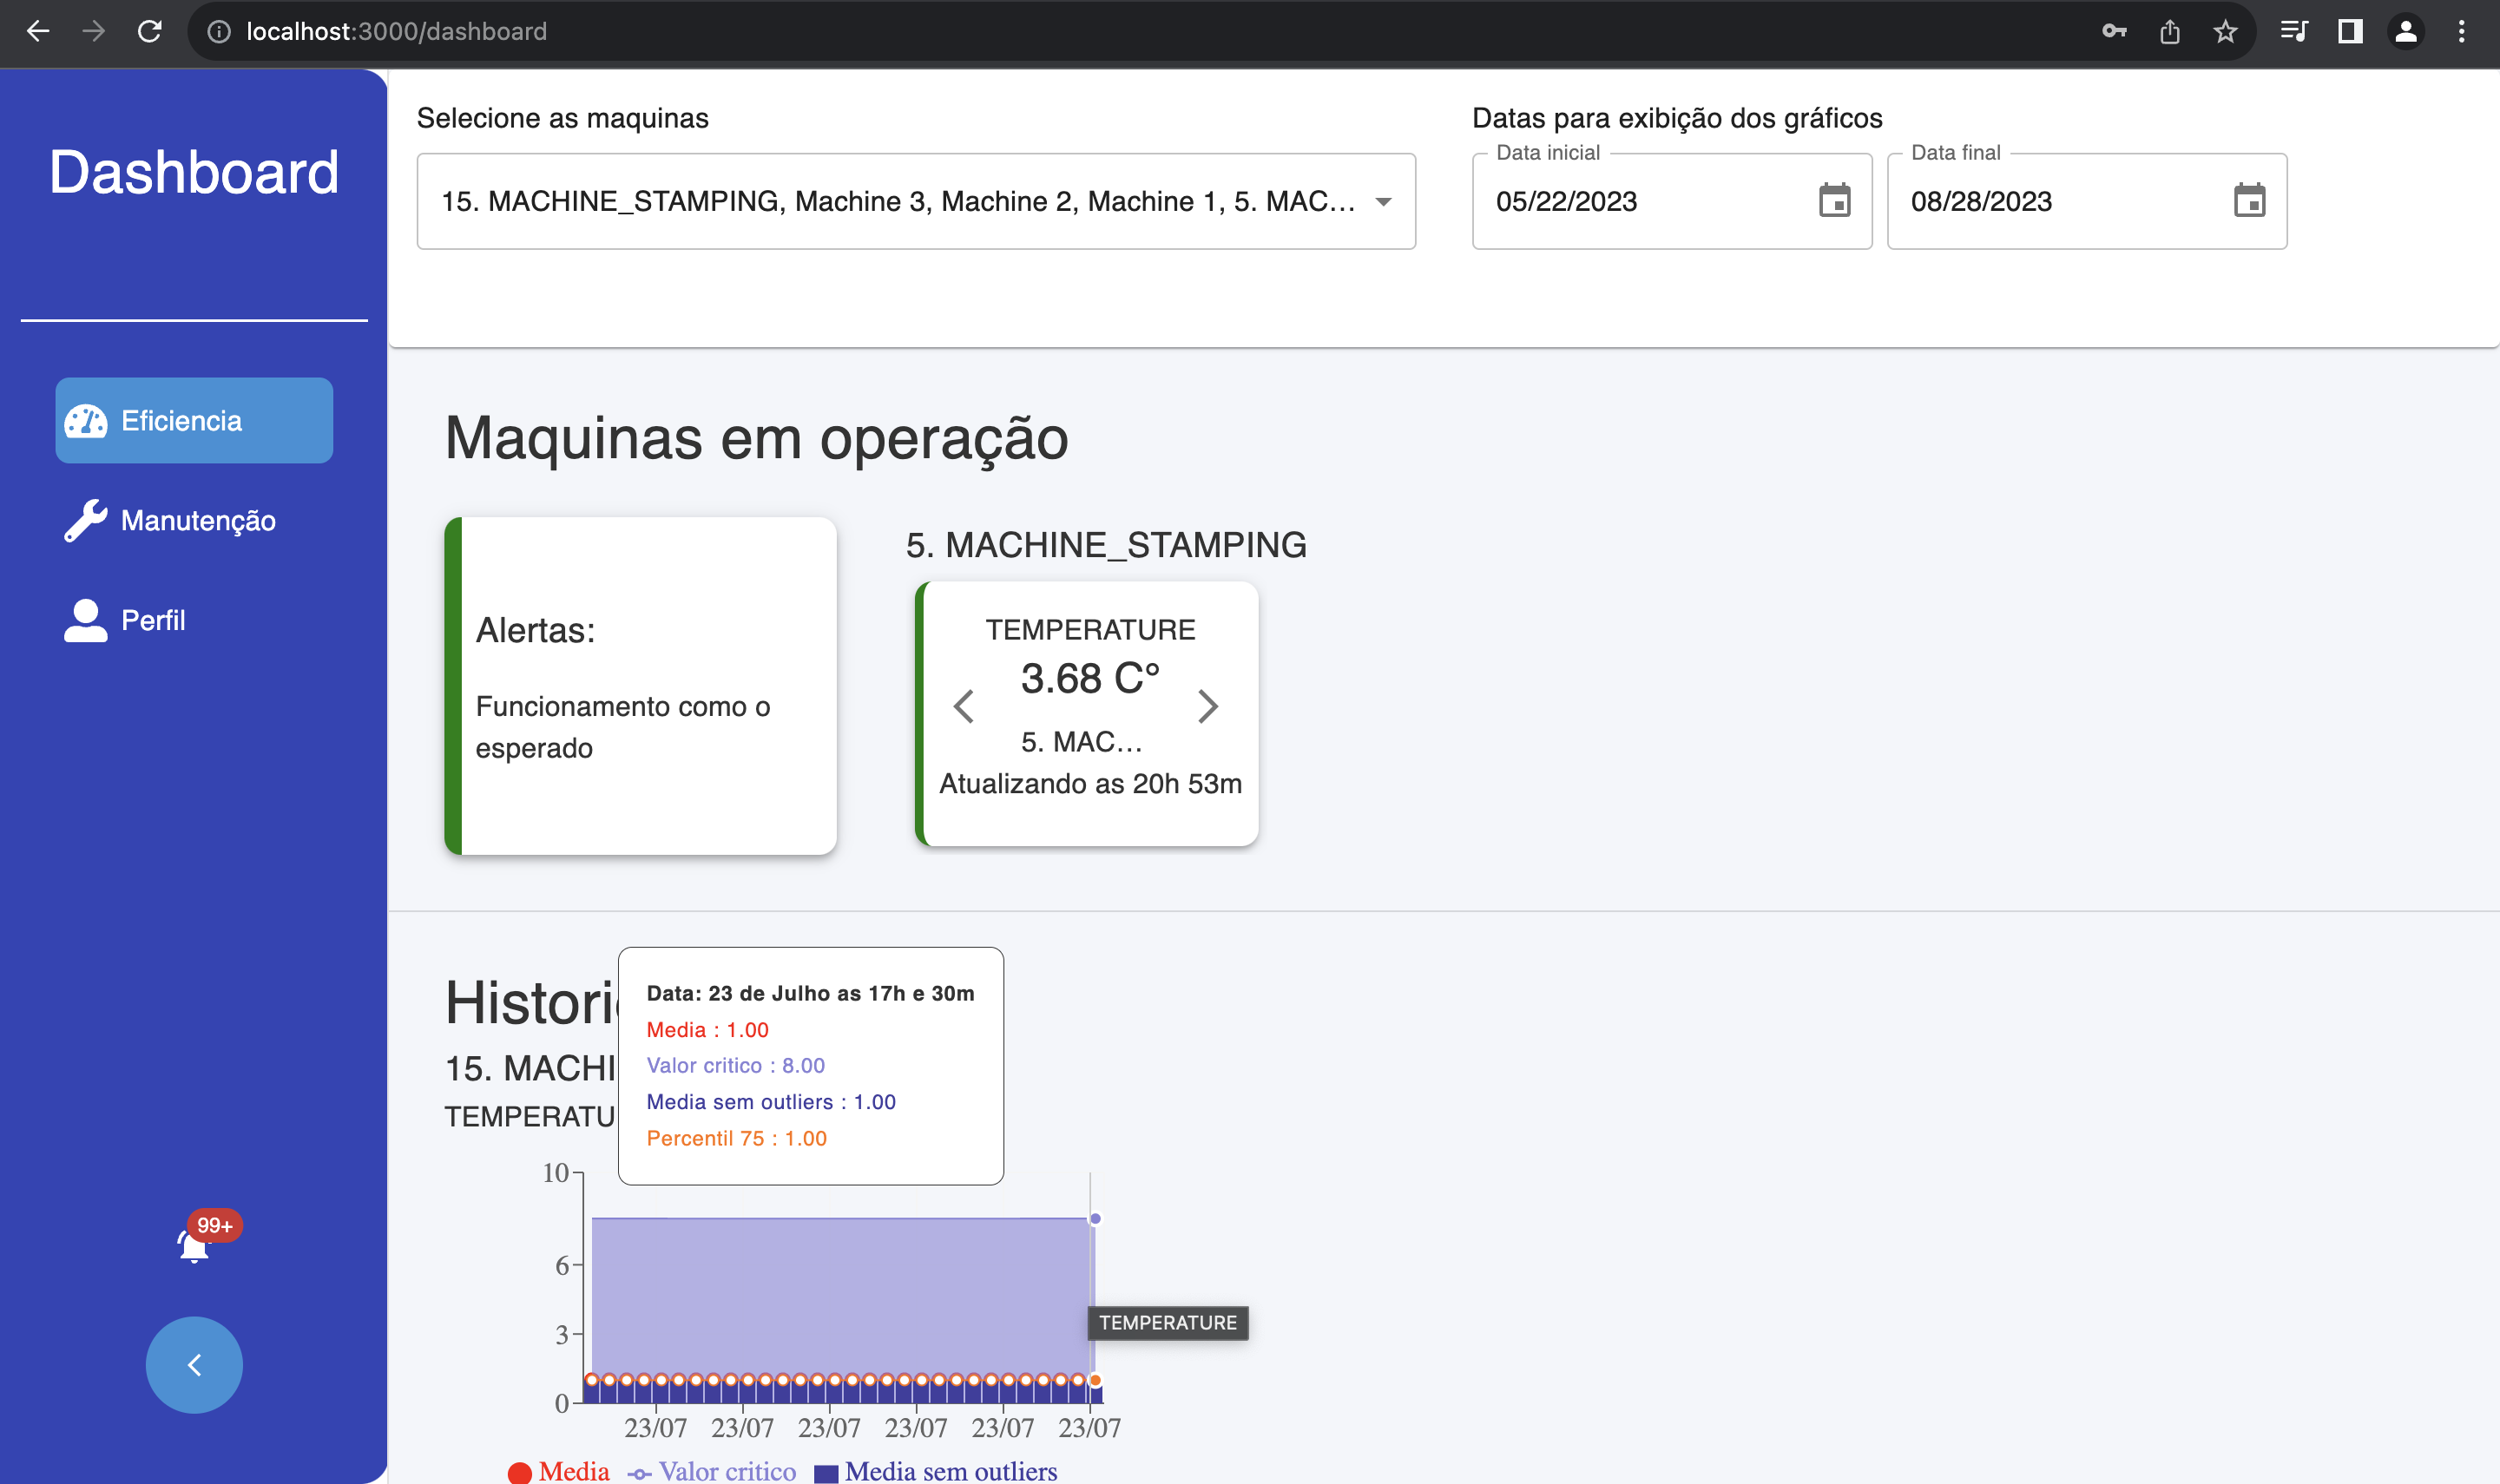
\includegraphics[width=0.7\textwidth]{images/dashboard.png}
	\caption{Dashboard with real time and graph data.}
	\label{fig:dashboradPage}
\end{figure}

No dashboard de interface do usuário são apresentados cartões individuais correspondentes a cada máquina monitorada, na figura \ref{fig:dashboradPage} pode ser visto essa página com um cartão da máquina \texttt{5. MACHINE\_STAMPING}. Em cada cartão, informações dos sensores são exibidas com a possibilidade de navegar entre elas com uma seta direcional. O cartão pode ser visto na figura \ref{fig:cardData}.

\begin{figure}[htbp]
	\centering
	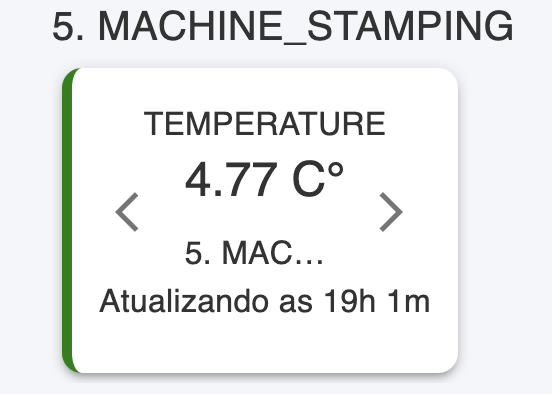
\includegraphics[width=0.4\textwidth]{images/machineCard.png}
	\caption{Card with machine data.}
	\label{fig:cardData}
\end{figure}

%TODO ref para a impl da camada de acesso externo do front
A obtenção desses dados em tempo real é efetuada através de um fluxo contínuo de dados por \textit{streaming}. O frontend da aplicação faz uma requisição ao endpoint \texttt{iot/realtime}, o qual retorna esse fluxo de dados em tempo real. A disponibilização dessa informação ocorre como explicado em X. 

%TODO ref para a impl do modulo de recebimento de dados
Na camada de backend, o fluxo de dados é constantemente alimentado pela classe \texttt{SensorValue}, que por sua vez, é atualizada pelo módulo de recebimento de dados. Ao receber novas leituras dos sensores, o módulo executa validações apropriadas antes de atualizar os valores na classe \texttt{SensorValue}, como explicado em X. Uma vez atualizada, a \gls{API} acessa esses novos valores e os insere no fluxo de dados transmitido ao usuário conectado.


\section[Alertas e notificações]{Alertas e notificações}\label{sec:alertsAndNotifications}

Esta funcionalidade tem como principal objetivo monitorar o desempenho das máquinas em tempo real e emitir alertas e notificações aos usuários caso sejam detectadas condições de operação inadequadas. Isso permite que ações corretivas sejam tomadas de forma imediata.

%TODO ref para a explicação de metadados
Sempre que uma nova leitura de sensor é recebida pelo módulo de recebimento de dados, uma validação é realizada para verificar se a máquina está operando dentro dos parâmetros aceitáveis. Esses parâmetros são obtidos através dos metadados do sistema, explicado em X.

Se um valor fora do intervalo aceitável é identificado durante a validação, o módulo de recebimento de dados insere uma marcação especial nessa leitura dentro da classe \texttt{SensorValue}. Essa marcação é posteriormente transmitida ao frontend durante o processo de transmissão de dados via \textit{stream}, como explicado em X. %TODO ref para a impl da transmissão em tempo real

Ao receber uma leitura marcada, o frontend atualiza o cartão de informação correspondente para refletir o estado anômalo. Especificamente, dentro do dashboard mostrado na figura \ref{fig:dashboradPage}, a cor do cartão é alterada para vermelho ou amarelo, tanto nos cards individuais, figura \ref{fig:cardData}, quanto no card geral que é usado para mostrar o status geral das maquinas, figura \ref{fig:geralMachineAlert}, portanto, servindo como um alerta visual imediato para o usuário. 

\begin{figure}[htbp]
	\centering
	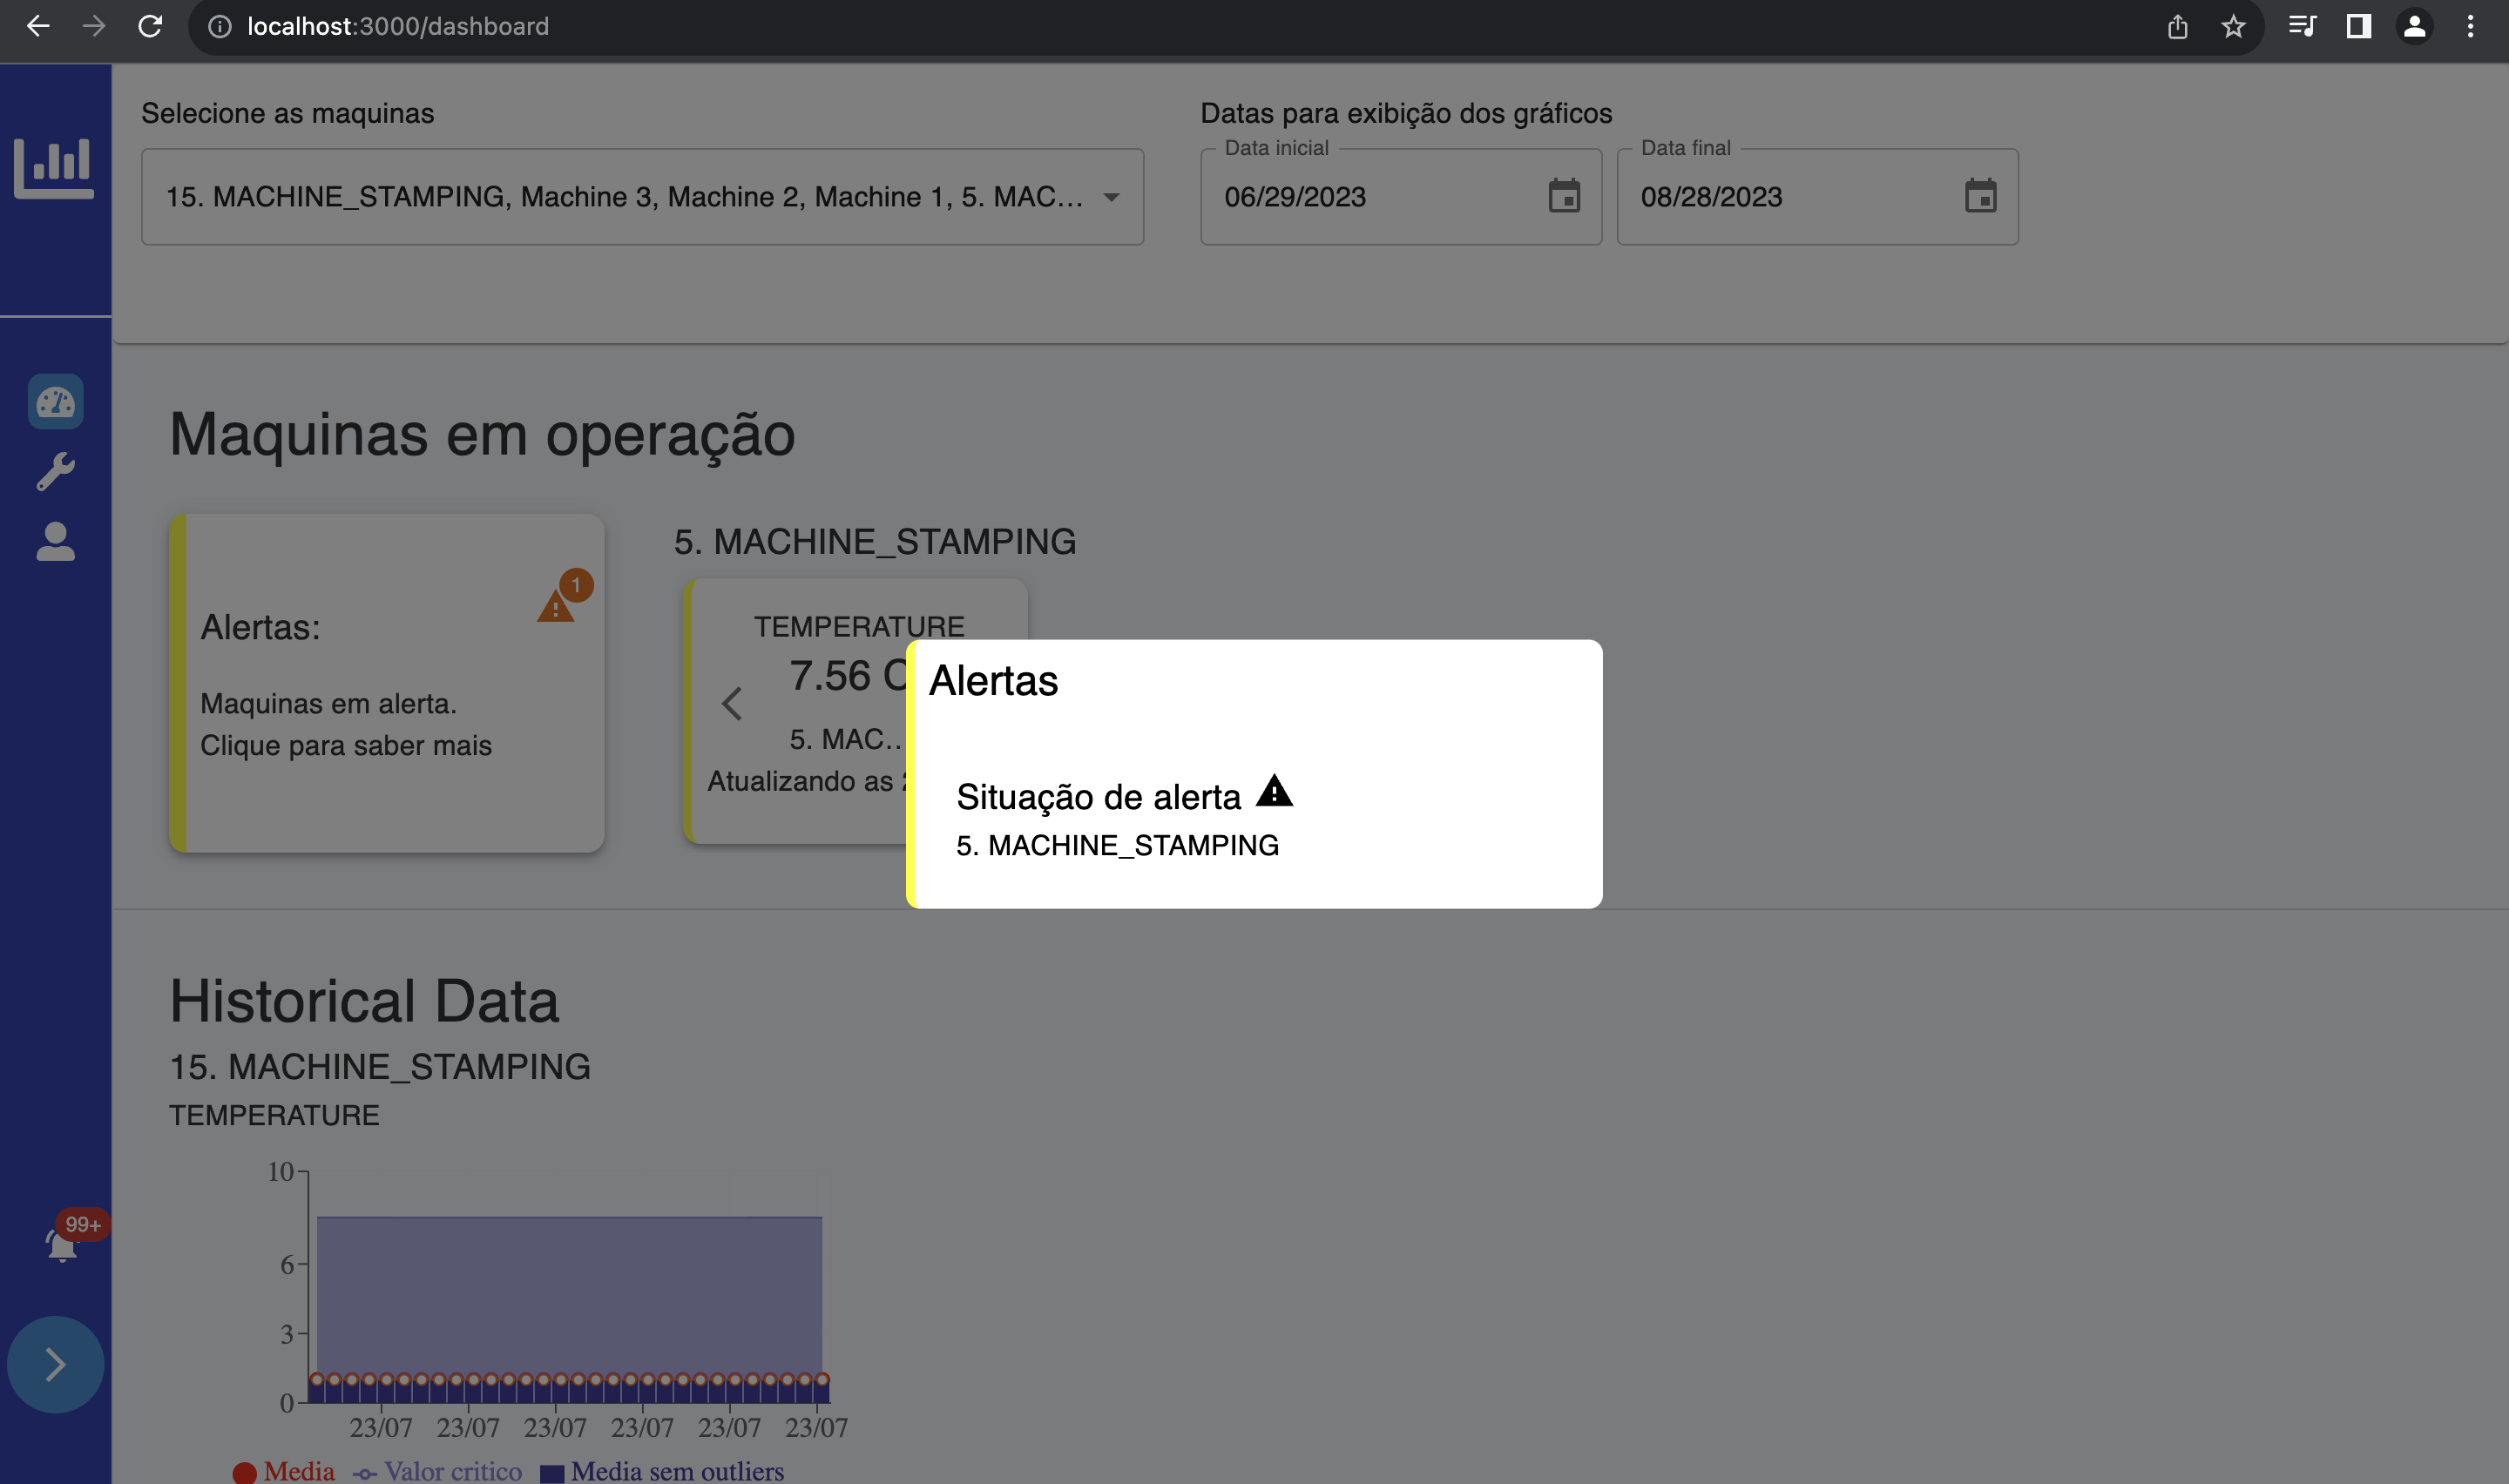
\includegraphics[width=0.8\textwidth]{images/geralMachineAlert.png}
	\caption{General Notifications.}
	\label{fig:geralMachineAlert}
\end{figure}

%TODO ref sub modulo de recebimento de dados que cuida dos alertas
O módulo de recebimento de dados, REF, mantém o controle do estado operacional de cada máquina que está enviando informações. Quando uma máquina sai de um estado de alerta, a ocorrência é registrada no banco de dados, com data de início e término do estado de alerta, junto com as informações referentes ao sensor e à máquina envolvida, como explicado em X. Posteriormente, uma mensagem é enviada aos usuários conectados utilizando a interface de \textit{WebSocket}, informando-os do mau funcionamento da maquina durante o período registrado pelo sistema. %TODO ref impl websocket

As informações sobre a finalização de alertas podem ser acessadas pelos usuários através de notificações na interface do sistema, como pode ser visto na figura \ref{fig:notificationDrawer}. Ao clicar no ícone de notificação no menu lateral do \textit{dashboard}, o usuário pode visualizar essas notificações.

\begin{figure}[htbp]
	\centering
	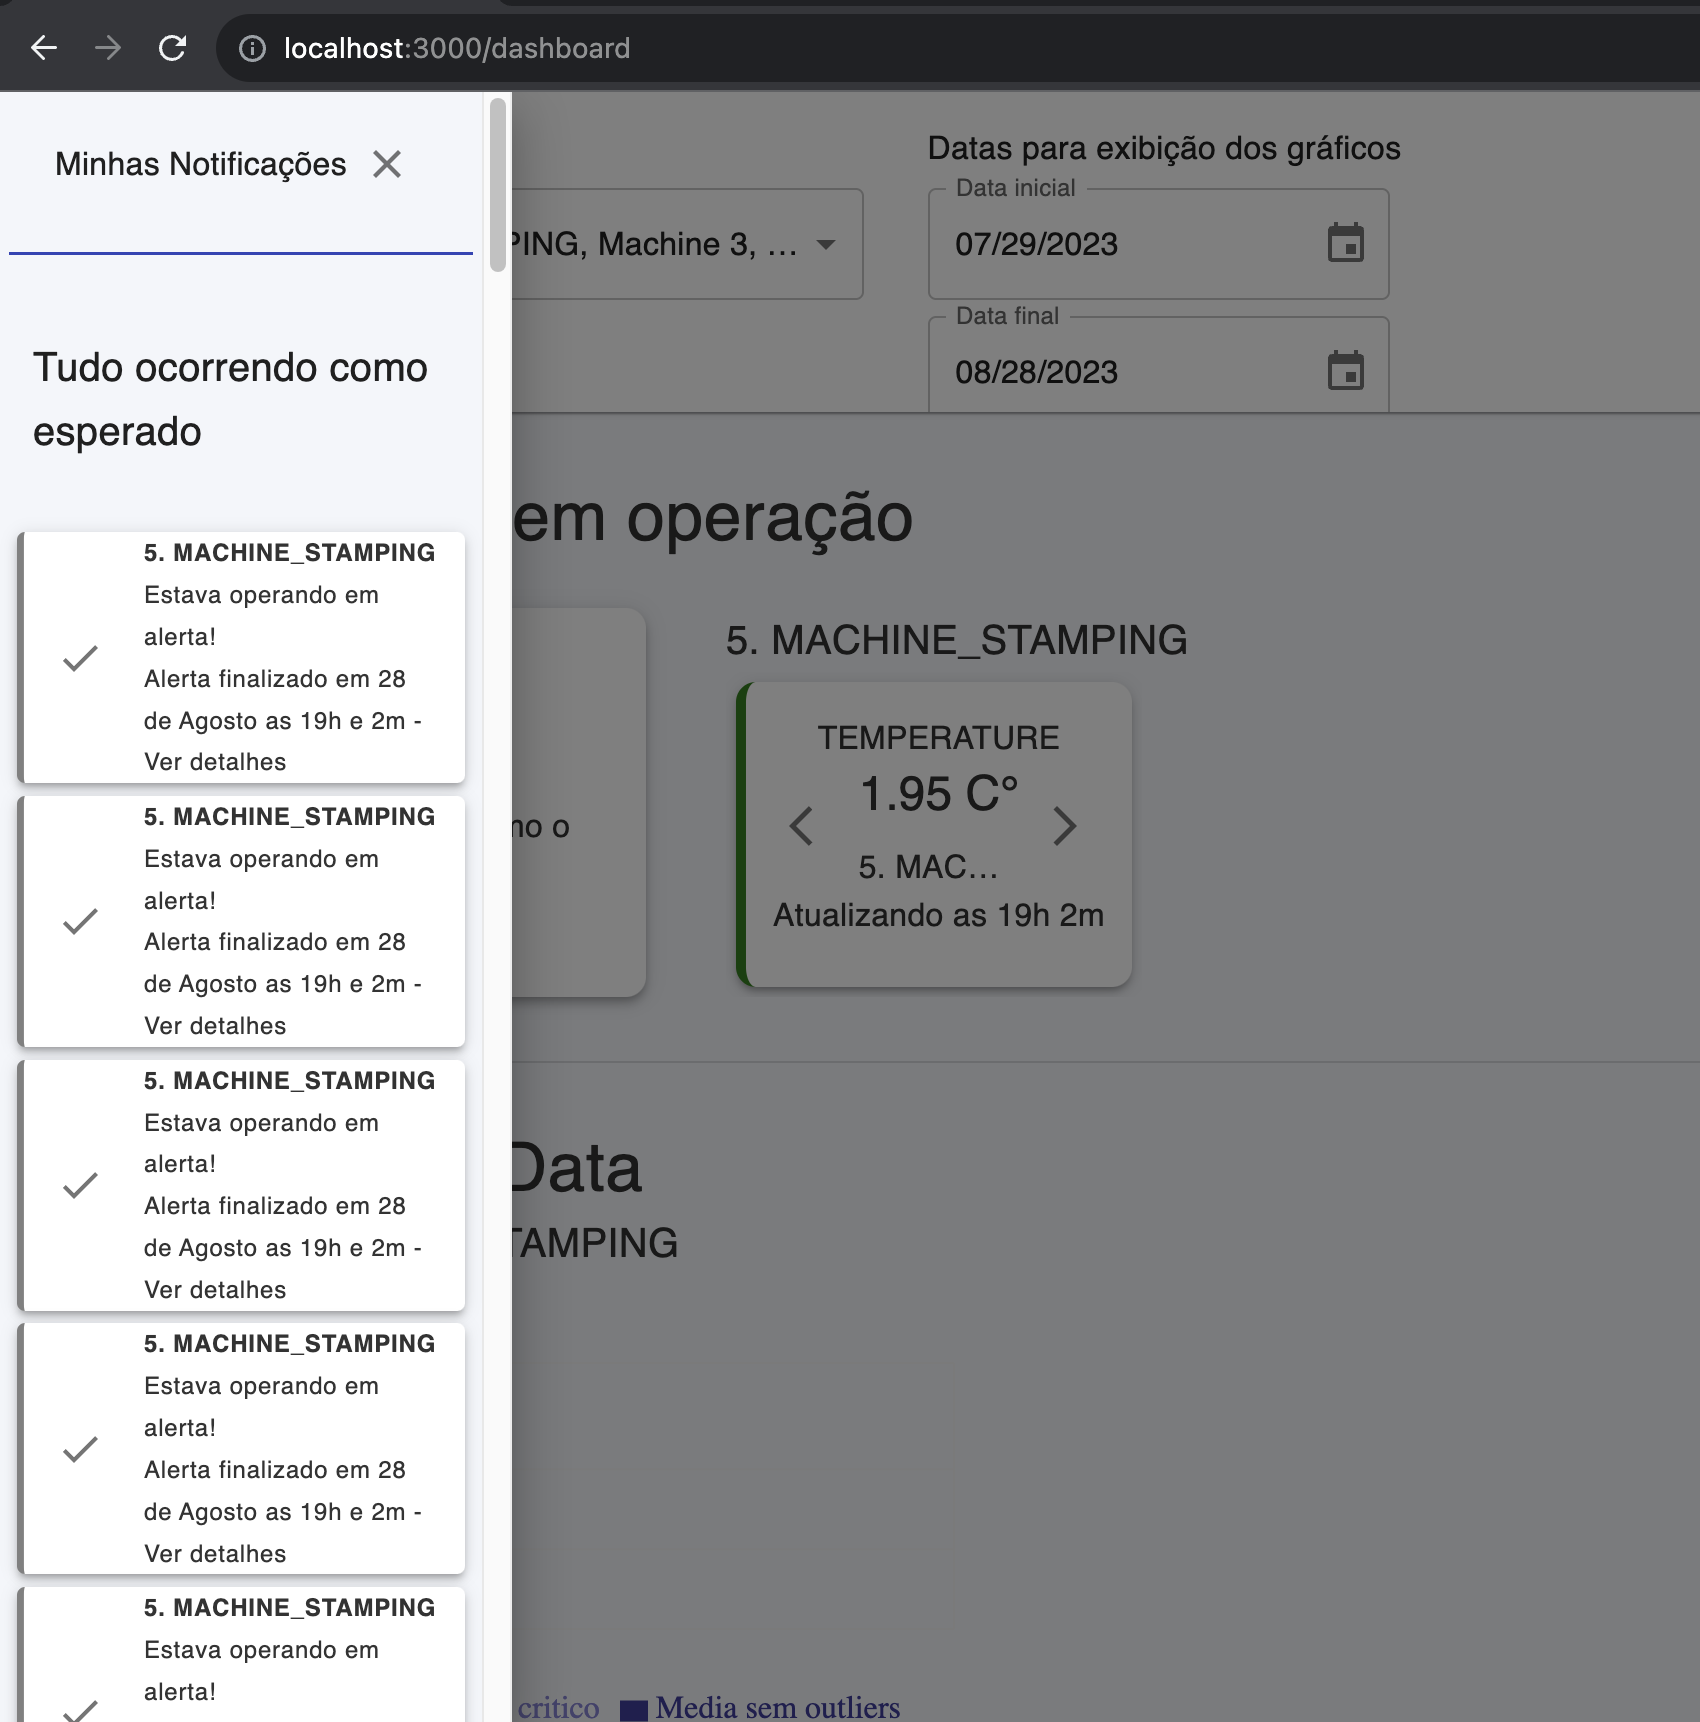
\includegraphics[width=0.6\textwidth]{images/notification.png}
	\caption{Notification drawer.}
	\label{fig:notificationDrawer}
\end{figure}


Portanto, ao iniciar uma sessão no sistema, as notificações anteriores são carregadas para o usuário. Além disso, qualquer nova notificação gerada durante a sessão do usuário é transmitida em tempo real por meio de uma conexão \textit{WebSocket} estabelecida entre o frontend e o backend, como explicado em X.%TODO ref impl websocket


\section[Analise estatística de dados históricos]{Analise estatística de dados históricos}\label{sec:histicalGraphs}

O módulo de processamento de dados é responsável pela análise estatística dos dados históricos. Seguindo o parâmetro padrão do sistema, todos os dias à meia-noite, os dados brutos não processados são lidos e analisados. O resultado da análise é então armazenado no banco de dados para consultas futuras, como explicado em X. %TODO ref modulo de processamento

A possibilidade de acessar esses dados analíticos é providenciada pela \gls{API}, especificamente pelo módulo "IOT Analytics". A requisição para obter essas informações deve ser autenticada, conforme descrito na seção "Módulos da API".%TODO ref impl API

A representação visual dessas análises é efetuada por meio de gráficos que agregam quatro métricas principais resultantes do processamento. Dessa forma é exibido no gráfico:

\begin{itemize}
    \item \textit{Valor Ideal}: Representado em um gráfico de área, serve como um parâmetro de funcionamento ideal para fornecer uma perspectiva relativa aos outros dados.
    \item \textit{Percentil 75}: Exibido em um gráfico de linha, esta métrica oferece uma visão sobre a distribuição dos valores durante o período de agregação e sua evolução ao longo do tempo.
    \item \textit{Média da Agregação}: Representada em um gráfico de dispersão, esta métrica fornece o valor médio dos dados agregados.
    \item \textit{Média com Remoção de \textit{Outliers}}: Ilustrada em um gráfico de barras, esta métrica é calculada após a remoção dos valores \textit{outliers}, conforme determinado pelo método de construção do boxplot.
\end{itemize}

Portanto, a imagem \ref{fig:graphData} mostra como fica a visualização dessas informações dentro do dashboard.

\begin{figure}[htbp]
	\centering
	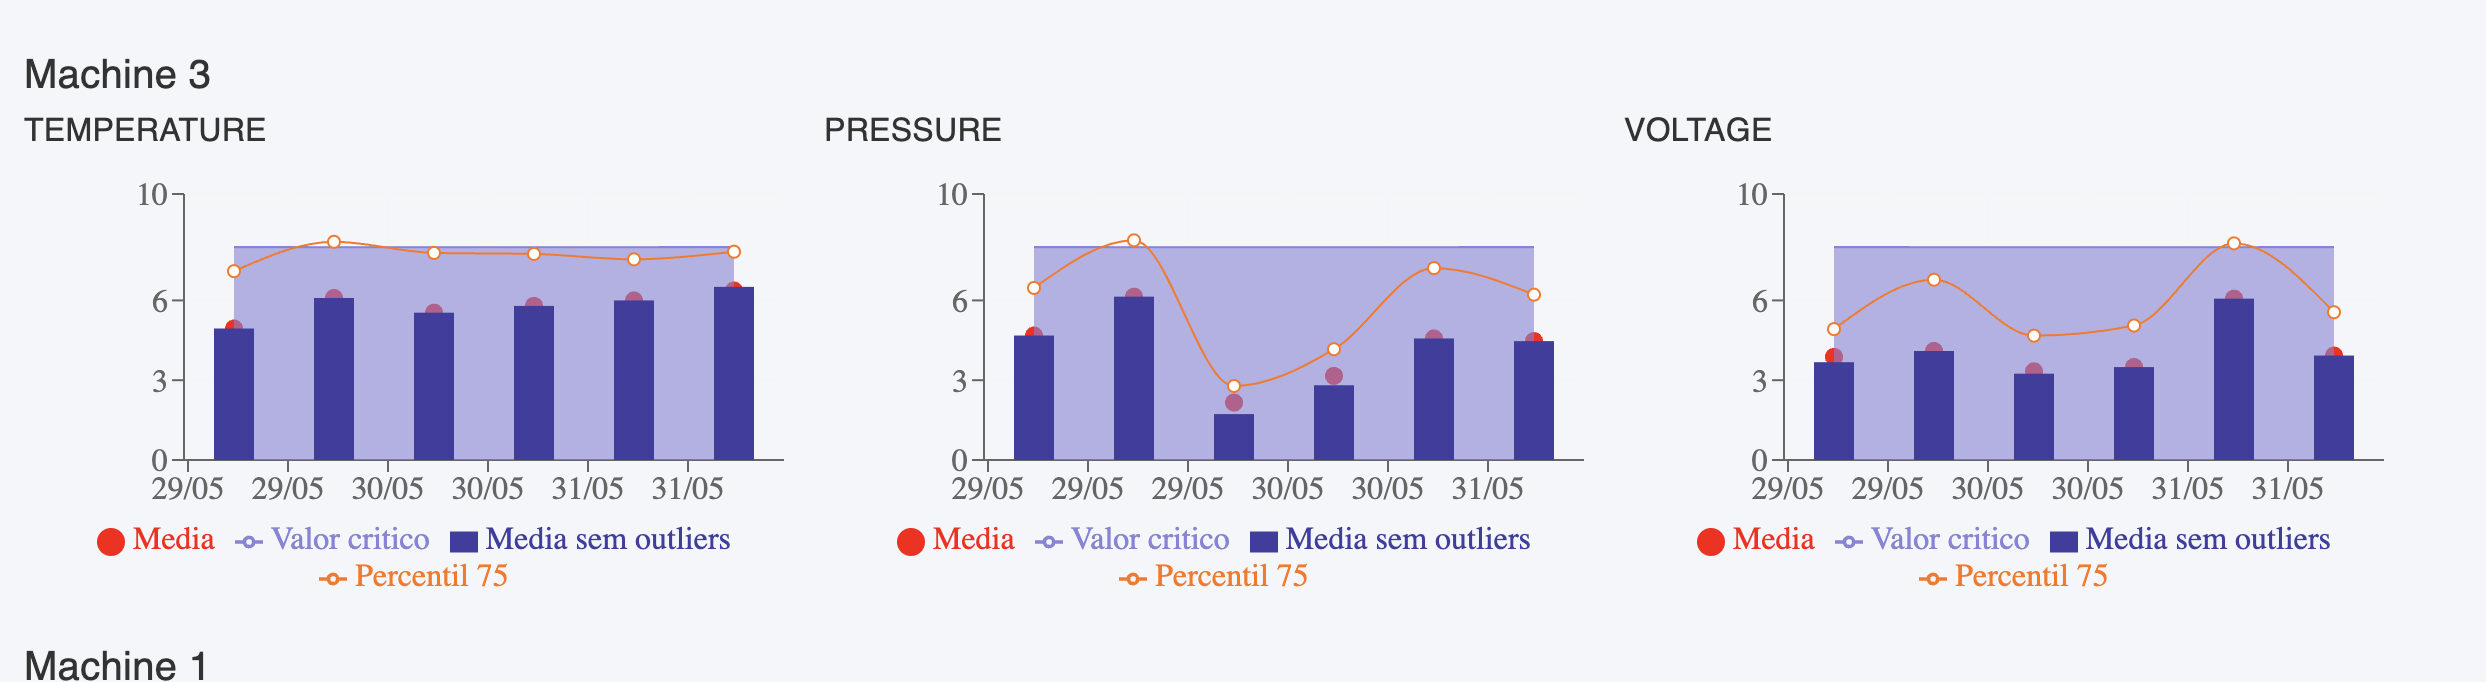
\includegraphics[width=0.7\textwidth]{images/graphData.png}
	\caption{Graph example.}
	\label{fig:graphData}
\end{figure}

\section[Exibição dos dados referente a paragem das máquinas]{Exibição dos dados referente a paragem das máquinas}\label{sec:downtime}

%TODO ref para a parte que explica melhor sobre isso XX
Esta funcionalidade é dedicada à exibição de dados relacionados às paragens das máquinas, armazenados previamente no banco de dados. Como esclarecido na seção XX, a funcionalidade tem o objetivo de demonstrar como seriam apresentados esses dados, caso fossem recebidos pelo sistema de forma similar aos dados dos sensores. A fonte dos dados para a elaboração desses gráficos provém de três planilhas recebidas no início do desenvolvimento do projeto, em que as informações foram salvas no banco de dados. Esses dados são acessados pelo frontend por meio do módulo \texttt{downtime\_analytics} da \gls{API}.

Os gráficos gerados para representar esses dados são apresentados na forma de gráficos de coluna. Cada gráfico exibe um título correspondente à planilha da qual os dados foram extraídos. A legenda do gráfico indica a porcentagem que cada parada específica representa em relação ao total de paragens.

Os gráficos de coluna fornecem uma maneira eficaz de comparar as diferentes paragens das máquinas, como pode ser visto na figura \ref{fig:downtime}. Esta visualização oferece um meio para analisar a eficiência operacional, identificar possíveis áreas para melhoria e acompanhar o resultado das ações tomadas em relação a paragem das máquinas e a manutenção preditiva.

\begin{figure}[htbp]
	\centering
	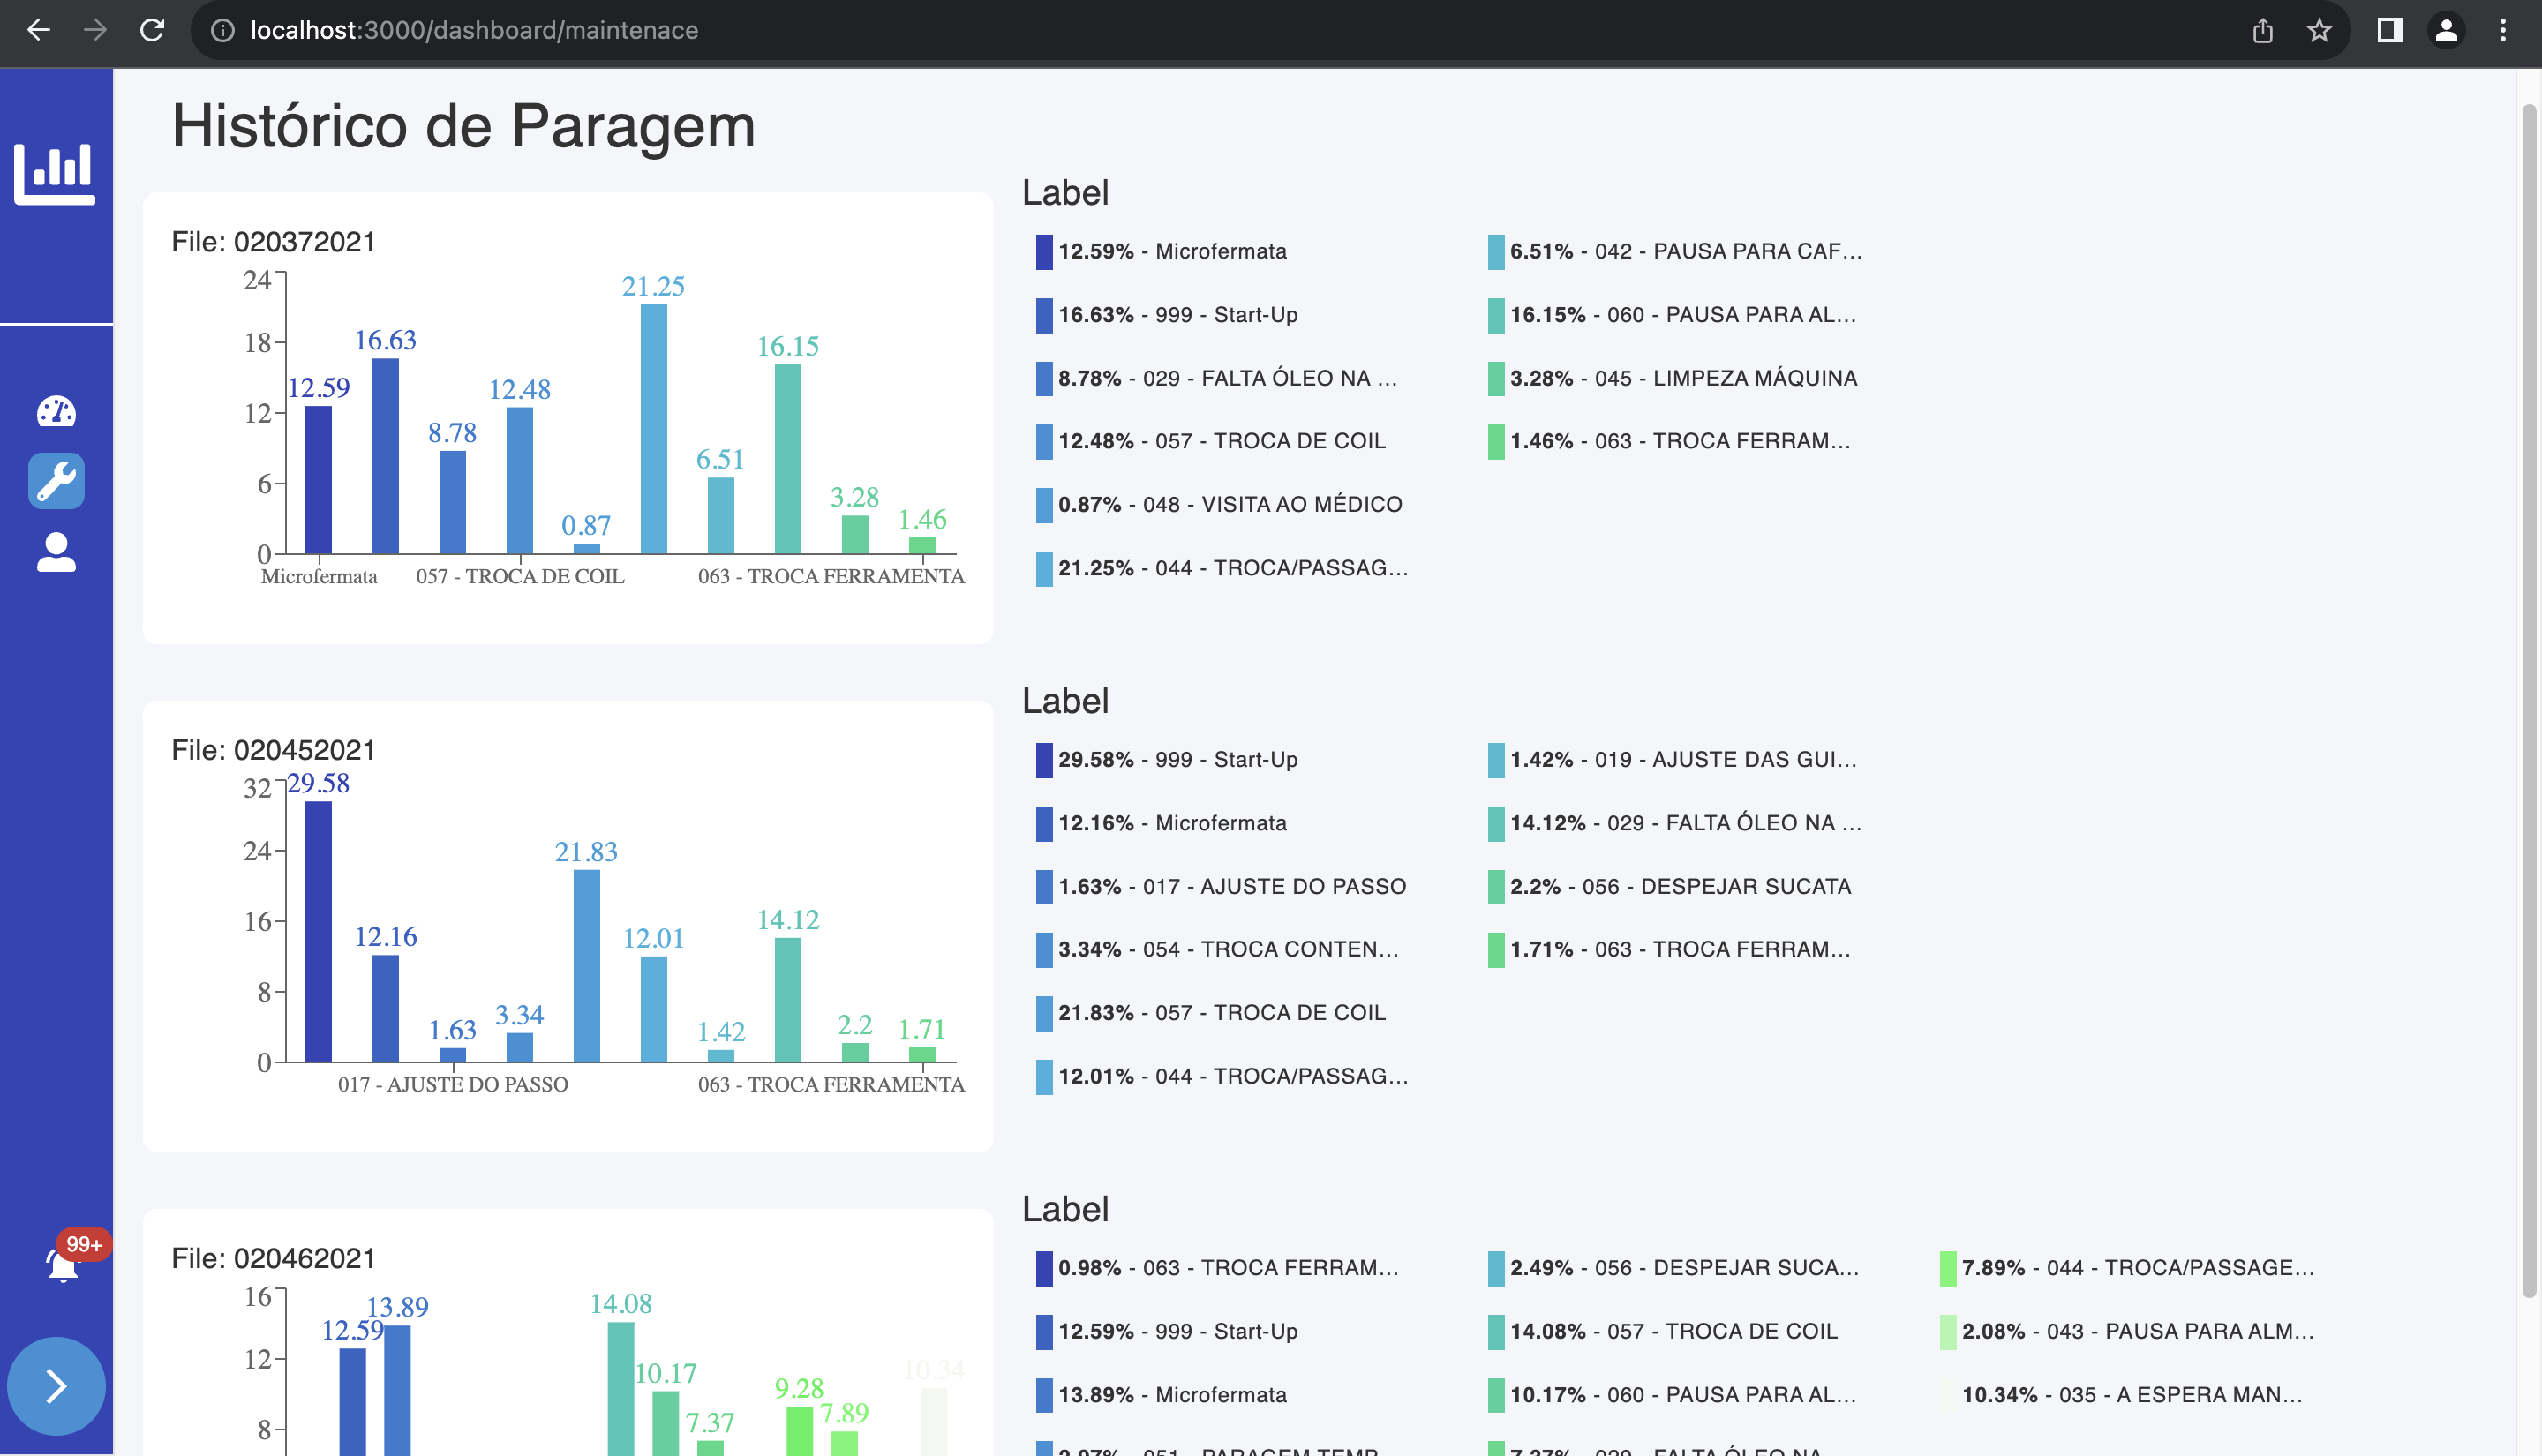
\includegraphics[width=0.75\textwidth]{images/downtime.png}
	\caption{Downtime graph.}
	\label{fig:downtime}
\end{figure}

\section[Perfil de usuário]{Perfil de usuário}\label{sec:profile}

A funcionalidade de perfil de usuário foi desenvolvida com o objetivo de fornecer aos usuários acesso aos seus dados pessoais armazenados no sistema. Além da visualização dessas informações, esta tela permite também a realização de modificações, incluindo a alteração de senha, e-mail e outros dados pessoais como nome, sobrenome e descrição.

%TODO ref para a parte de modulos da API
Para ler e modificar os dados apresentados, o módulo \textit{User} da \gls{API} é utilizado REF. Este módulo disponibiliza endpoints que permitem o acesso e a modificação dos dados armazenados, garantindo que as informações sejam atualizadas conforme as interações do usuário, como pode ser visto na figura \ref{fig:profilePage}.

Um recurso adicional fornecido por esta tela é a opção de logout. Ao selecionar esta opção, todas as informações armazenadas do lado do cliente são apagadas, efetuando assim a saída segura do usuário do sistema.

\begin{figure}[htbp]
	\centering
	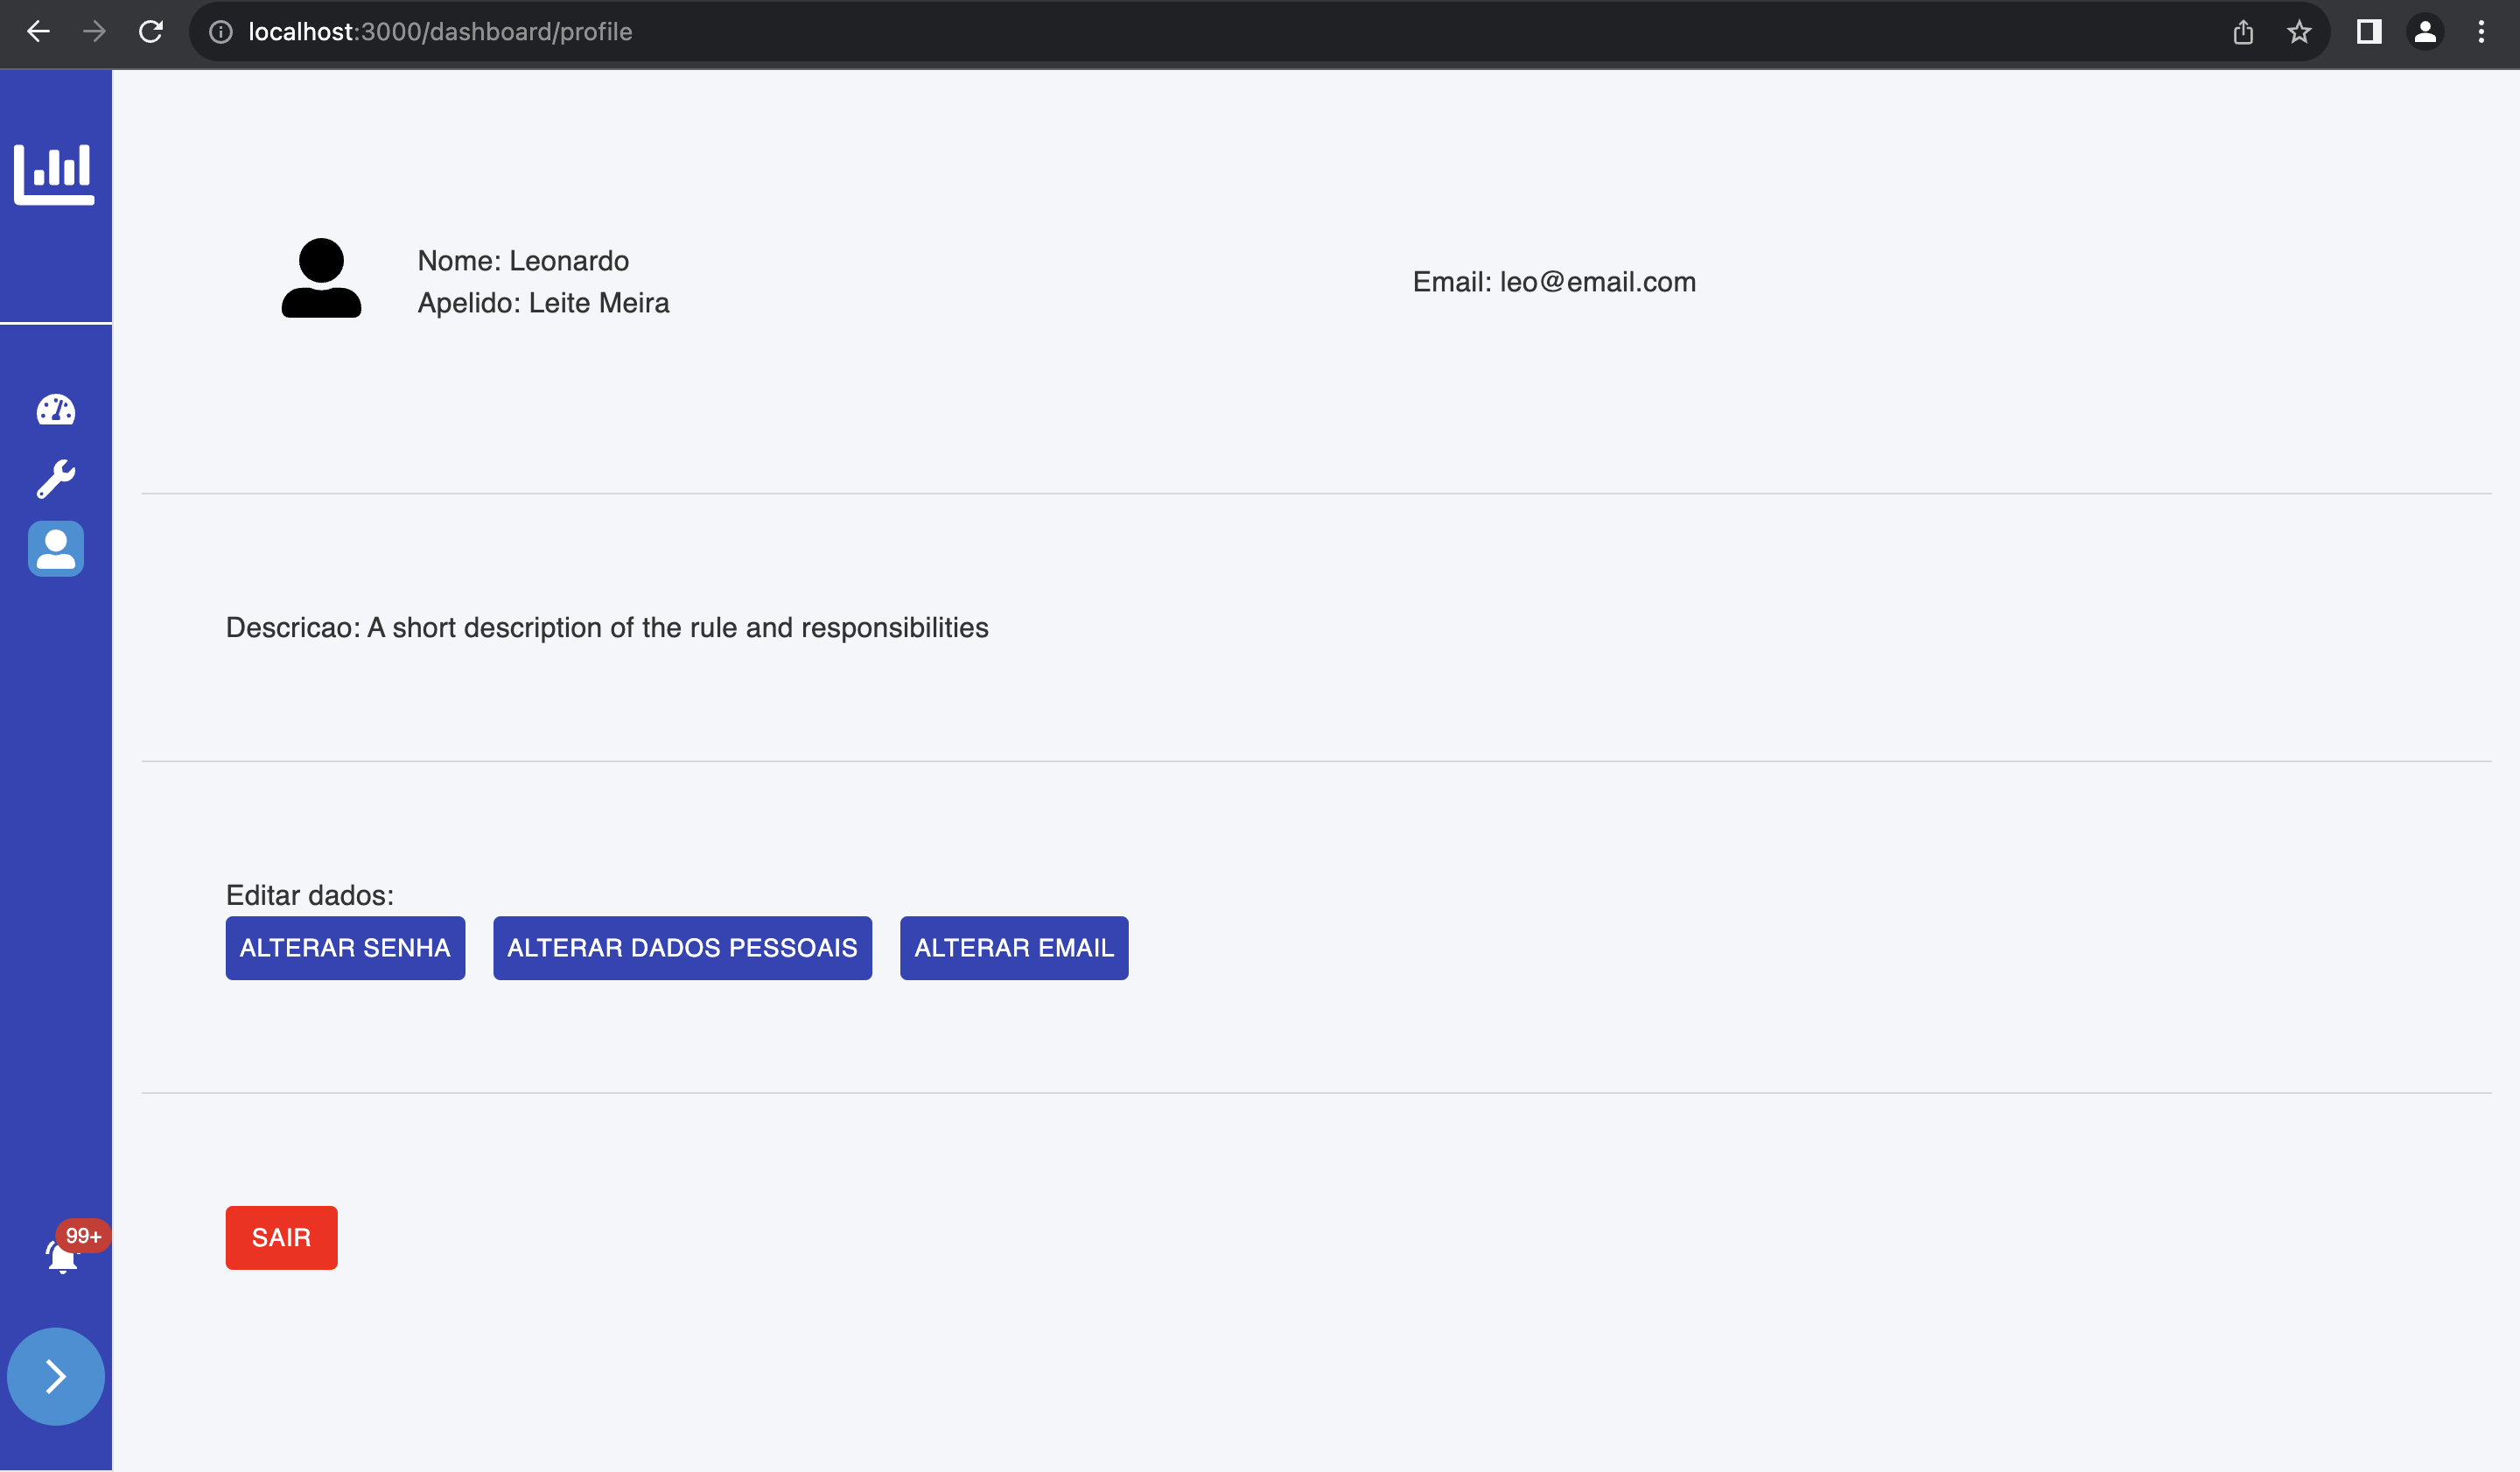
\includegraphics[width=0.8\textwidth]{images/profile.png}
	\caption{Profile page.}
	\label{fig:profilePage}
\end{figure}


\chapter{Resultados e Avaliação}\label{cap:results}
%TODO ref para um artigo com vantagens de usar um sistema de monitoramento em tempo real
Neste capítulo, será apresentada uma avaliação do sistema desenvolvido, focando em seus benefícios e vantagens competitivas, bem como os resultados de testes e validações realizadas. O sistema pode ser modificado de tal forma que pode ser adaptado para outros contextos, onde informações geradas por sensores necessitam ser visualizadas em tempo real, e onde o processamento e análise de dados históricos são requeridos.

A implementação deste sistema pode auxiliar na identificação mais rápida de problemas na produção, graças ao monitoramento em tempo real. Além disso, os insights gerados pela análise histórica de dados podem ser instrumentalizados para otimizar processos de produção. 

%TODO ref para artigo diferencia competitiva para gestão orientada a dados
A adoção de um sistema como este representa uma vantagem competitiva, potencialmente elevando a eficiência da empresa em relação à concorrência. No entanto, é importante observar que o software ainda não foi implementado em um ambiente de produção, e portanto, existe um conjunto ainda não mapeado de melhorias que devem ser realizadas para que o sistema opere da forma mais eficaz possível.


\section{Benefícios}\label{sec:benfits}

Uma série de benefícios é oferecida pelo sistema desenvolvido. Em primeiro lugar, o monitoramento abrangente das máquinas em toda a planta industrial é facilitado. Por meio deste monitoramento, informações cruciais sobre o estado operacional de cada máquina são exibidas para os funcionários em tempo real.

Adicionalmente, o sistema proporciona a capacidade de tomar ações mais rápidas em caso de problemas operacionais, e como resultado, o tempo improdutivo das máquinas pode ser reduzido, mitigando prejuízos associados à produção.

%TODO ref para artigo de gestão orientada a dados
Outro aspecto vantajoso reside na avaliação de eficácia das medidas de manutenção implementadas. Por meio de acompanhamento histórico, o sistema permite visualizar os efeitos de ações tomadas para a manutenção das máquinas, deste modo, decisões mais informadas e efetivas podem ser tomadas rapidamente, ampliando os benefícios para outras máquinas na planta.

Finalmente, os dados históricos do sistema contribuem também para a geração de insights a partir da sua análise. Esta análise pode fornecer uma nova perspectiva para monitorar o desempenho das máquinas, e anomalias operacionais podem ser identificadas e medidas corretivas específicas podem ser implementadas para melhorar determinados indicadores.

\section{Vantagens competitivas}\label{sec:competitive}
O sistema desenvolvido oferece um conjunto de vantagens competitivas que se manifestam principalmente quando contrastadas com empresas que não implementam uma solução similar. Inicialmente, a falta de um sistema de monitoramento adequado pode resultar em operações abaixo do potencial eficiente para uma empresa. Este cenário gera custos adicionais em manutenção, perda de equipamentos e até mesmo desperdício de materia prima.

%TODO ref para artigo de gestão orientada a dados - redução de custos
Por outro lado, a implementação de um sistema de monitoramento robusto, proporciona benefícios à eficiência da produção, manutenção e desenvolvimento de produtos e serviços. O monitoramento em tempo real e a análise de dados históricos permitem a otimização de várias operações, desde a identificação rápida de problemas até a implementação de ações corretivas e preventivas. 

%TODO ref para artigo de gestão orientada a dados - melhoria da operação, preço e qualidade do serviço
Deste modo, a qualidade dos produtos ou serviços é significativamente melhorada. Além disso, as informações geradas podem ser utilizadas para uma produção mais enxuta e eficiente, o que reduz os custos gerais e, por consequência, pode tornar o produto ou serviço mais competitivo em termos de preço.

Portanto, as vantagens competitivas geradas pelo uso deste sistema são multifacetadas, englobando não apenas a eficiência operacional, mas também a qualidade e o custo de produtos e serviços. Essas melhorias conjuntas possibilitam que a empresa adquira uma posição mais sólida e vantajosa no mercado em que atua.

\section{Realização de testes e validações}\label{sec:tests}

%TODO Ref para artigo com a importancia de testar o software em ambiente produtivo
Embora todos os requisitos levantados para o sistema tenham sido atendidos e as histórias de usuários detalhadas tenham sido completadas, uma avaliação significativa do sistema em um ambiente de produção ainda não foi realizada. A importância de testar e validar um sistema de software em um ambiente real não pode ser subestimada, pois a realização de testes é fundamental para avaliar a adequação do sistema às necessidades práticas, enquanto a validação assegura que o sistema cumpre os requisitos estabelecidos. 

%TODO ref para artigo sobre as etapas ideias de desenvolvimento de software
%TODO ref para artigo sobre influencia de um sistema top-down ou cascata para testar
O desenvolvimento de sistemas de software é um processo iterativo que envolve uma série de etapas, incluindo requisitos, design, implementação, testes e manutenção. Cada uma dessas etapas requer revisão e ajustes com base nos resultados dos testes e validações. A falta de uma etapa rigorosa de testes e validações pode resultar em várias deficiências, tanto técnicas quanto funcionais, que podem não apenas afetar o desempenho do sistema, mas também torná-lo impraticável para uso em um ambiente de produção.

Sem uma série adequada de testes, o sistema é susceptível a falhas que podem ser tanto técnicas, como relacionadas aos requisitos funcionais. Estas falhas podem ser pequenas, mas têm o potencial de escalonar e comprometer a integridade do sistema. Assim, a ausência de testes e validações em um ambiente real representa uma lacuna importante que deve ser abordada para assegurar a robustez e eficácia do sistema.

\cleardoublepage
\chapter{Conclusão e Trabalhos Futuros}\label{chap:conclusion_and_future_work}

O capítulo está estruturado nas seções "Resumo" do projeto, uma discussão sobre as "Limitações do Sistema" e finalmente, "Sugestões para Trabalhos Futuros". 

A construção do sistema é considerada bem-sucedida, servindo como um marco inicial para futuras implementações e adaptações. Os próximos passos para o avanço deste projeto incluem a colocação do sistema em um ambiente de produção, seguida pela coleta de feedback de usuários. Esta abordagem permitirá um processo incremental de aprendizagem, no qual o sistema será constantemente aprimorado com base nas experiências adquiridas e nas necessidades identificadas. 

\section{Resumo}\label{sec:summary}
Nesta dissertação, foi desenvolvido um sistema multifuncional destinado à coleta, armazenamento, processamento e visualização de dados gerados por sensores. Utilizou-se Python para a criação da \gls{API} e do módulo de processamento, MongoDB para o gerenciamento do banco de dados e NextJs para a construção do painel de controle, conhecido como \emph{dashboard}. A arquitetura do sistema pode ser vista em \ref{cap:development}.

Os dados foram recebidos através de uma conexão multicast estabelecida pelo módulo de recebimento de dados, mostrado em \ref{subsec:receiveDataModuleArch}. Uma vez recebidos, os dados foram imediatamente submetidos a uma análise preliminar para identificar qualquer condição que pudesse acionar um alerta. Caso um alerta fosse gerado, os usuários eram notificados, permitindo intervenções rápidas e eficazes.

Para a análise de dados históricos, empregou-se o método BoxPlot no módulo de processamento, explicado em \ref{subsec:moduloProcessamento}. Esta análise objetivou a identificação de padrões e anomalias nos dados coletados ao longo do tempo, fornecendo insights valiosos para a operação e manutenção das máquinas monitoradas.

A \gls{API}, descrita em \ref{sec:api}, desempenhou um papel crucial no sistema, gerenciando o acesso aos dados. A segurança foi assegurada através da implementação de autenticação por \gls{JWT}, e vários \emph{endpoints} foram desenvolvidos para permitir um acesso eficaz aos dados.

O \emph{frontend}, descrito em \label{sec:implFront},por sua vez, foi responsável por exibir informações em tempo real, alertas gerados e dados processados em forma de gráficos.

\section{Limitações do Sistema}\label{sec:limitations}

Apesar dos avanços alcançados com o desenvolvimento do sistema em questão, algumas limitações foram identificadas que poderiam influenciar sua eficácia e aplicabilidade em diferentes contextos.

Primeiramente, identifica-se que o módulo de recebimento de dados necessita ser adaptado especificamente para cada contexto operacional. Esta exigência pode comprometer a portabilidade do sistema, exigindo ajustes manuais sempre que uma nova aplicação é considerada.

Em segundo lugar, existem restrições em relação à estrutura dos dados recebidos, pois para o funcionamento eficaz do módulo de recebimento de dados e da funcionalidade de alerta, é necessário que os dados recebidos possuam um campo de identificação e um valor numérico correspondente. A ausência deste último impede que os alertas sejam identificados e torna o módulo de processamento ineficaz para a análise desses dados.

Por último, o sistema foi projetado e testado em um ambiente com uma quantidade limitada de máquinas conectadas. Não foram realizados testes para avaliar o desempenho do sistema sob a carga de uma grande quantidade de máquinas e sensores enviando dados simultaneamente. Portanto, para cenários com maior escala, adaptações podem ser necessárias para assegurar o desempenho e a eficácia do sistema.


\section{Sugestões para Trabalhos Futuros}\label{sec:future_work}

Com base nas observações e análises realizadas ao longo deste projeto, existem diversos trabalhos que podem ser feitos no sistema para pesquisa e desenvolvimento futuro.


\subsection{Utilização de inteligencia artificial para predição}

Dado que os dados lidos pelos sensores são armazenados no sistema, eles têm o potencial de revelar informações significativas sobre o funcionamento das máquinas. A aplicação de técnicas de \gls{AI} aos dados coletados foi identificada como a principal funcionalidade para a evolução do sistema, que pode se tornar uma ferramenta robusta para manutenção preditiva. Ao aplicar algoritmos de aprendizado de máquina aos dados armazenados, podem ser gerados modelos preditivos que antecipam falhas ou ineficiências em equipamentos industriais.

A implementação de um sistema de manutenção preditiva baseado em \gls{AI} poderia conferir uma vantagem competitiva significativa à empresa, não apenas melhoraria a eficiência operacional, mas também otimizaria a alocação de recursos para manutenção, resultando em redução de custos e aumento de produtividade. Portanto, a exploração futura de \gls{AI} para a análise de dados armazenados é fortemente recomendada para aprimorar a eficácia do sistema em estudo.

\subsection{Monitoramento e Logs}

O monitoramento abrangente do sistema e a manutenção de logs de atividades são aspectos cruciais para a sustentabilidade e escalabilidade do sistema. A ausência de um sistema de logs bem estruturado pode resultar em dificuldades na identificação e resolução de problemas que podem surgir durante o funcionamento do sistema em tempo real. Nesse contexto, três áreas principais são identificadas onde o monitoramento e os logs poderiam fornecer insights valiosos para aprimoramento contínuo.

Além disso, seria vantajoso manter um registro abrangente das transações de dados entre os sensores e o módulo de recebimento de dados. Esses logs poderiam incluir informações como data e hora da transação, identificação do sensor, e qualquer anomalia ou falha durante o processo de recebimento. Isso facilitaria a verificação da integridade dos dados recebidos e ajudaria na detecção precoce de possíveis problemas no hardware ou na conectividade da rede.

\subsubsection{Log para Análise Estatística}

O módulo de processamento de dados, responsável pela análise estatística, também seria beneficiado por um sistema de logs. Detalhes sobre a execução do BoxPlot ou qualquer outra análise estatística poderiam ser registrados. Isso inclui informações como o número de pontos de dados analisados, quaisquer outliers detectados, e o tempo levado para a execução da análise. Com essas informações, seria possível refinar mais o algoritmo de análise e identificar áreas para otimização.

\subsection{Parâmetros Dinâmicos para Alertas}

Na versão atual do sistema, os parâmetros responsáveis por disparar alertas são definidos de forma estática, incorporados diretamente no código-fonte. Essa abordagem, embora funcional, apresenta limitações em termos de flexibilidade e adaptabilidade a diferentes cenários operacionais.

Na configuração atual, qualquer alteração nos parâmetros de alerta exige uma intervenção direta no código, seguida de um processo de teste e implantação, que pode ser tanto demorado quanto propenso a erros. Além disso, a falta de flexibilidade limita a capacidade da empresa de adaptar-se rapidamente a novas condições operacionais.

Seria vantajoso permitir que os parâmetros de alerta sejam configurados de forma dinâmica, através da interface de usuário do sistema. Uma funcionalidade que permita aos usuários ajustar os limiares de alerta e outros parâmetros relacionados poderia ser implementada. A possibilidade de fazer esses ajustes em tempo real, sem a necessidade de interromper o funcionamento do sistema, representaria um avanço significativo na usabilidade e adaptabilidade do sistema.

Com a implementação de parâmetros dinâmicos, os usuários poderiam responder mais rapidamente às mudanças nas condições operacionais, como variações na carga de trabalho das máquinas ou atualizações nas políticas de segurança. Além disso, essa flexibilidade aumentaria a portabilidade do sistema, facilitando sua implantação em diversos ambientes industriais com requisitos distintos.

\subsection{Generalização para Outros Contextos}

O sistema desenvolvido foi projetado inicialmente para um ambiente industrial específico. Embora eficaz nesse contexto, a transferência direta do sistema para outras áreas industriais pode não ser trivial. Portanto, a generalização do sistema para outros contextos é identificada como uma área de interesse para trabalhos futuros.

O módulo de recebimento de dados atualmente requer personalização específica para cada contexto industrial. Além disso, o sistema foi projetado para analisar dados que contêm um campo de identificação e um valor numérico. A falta desses campos poderia dificultar ou inviabilizar a adaptação do sistema em ambientes que exigem o tratamento de diferentes tipos de dados.

Pesquisas futuras poderiam explorar métodos para tornar o módulo de recebimento de dados e o módulo de processamento mais flexíveis e adaptáveis a diferentes tipos de dados e estruturas. Técnicas de aprendizado de máquina ou métodos estatísticos avançados poderiam ser aplicados para automatizar a detecção de eventos anômalos em diferentes cenários, sem a necessidade de programação manual extensiva.

%TODO ref para industria 4.0
%TODO ref para artigo que mostra que o uso de dados está mais critico e mandatório para as empresas
A capacidade de adaptar o sistema para diferentes contextos industriais não só aumentaria sua aplicabilidade, mas também poderia levar a melhorias na eficiência de operações industriais em uma variedade de setores. Isso é particularmente relevante em um cenário em que a indústria 4.0 e a Internet das Coisas estão ganhando impulso, e a análise de dados em tempo real torna-se cada vez mais crítica para a competitividade empresarial.

\subsection{Otimização de Performance}

A capacidade do sistema de escalar e operar eficientemente sob carga elevada não foi amplamente testada. Em particular, há preocupações relativas ao desempenho quando um grande número de máquinas está conectado e enviando dados simultaneamente, bem como à capacidade do frontend de exibir múltiplos dados em tempo real.

O sistema ainda não foi colocado em produção, portanto também não foi avaliado em um ambiente com tráfego elevado, tanto em termos de máquinas conectadas quanto de usuários acessando o dashboard. Portanto, os desafios associados à escalabilidade, como latência no recebimento de dados e possíveis gargalos na base de dados, ainda são desconhecidos.

O frontend, construído em Next.js, tem o potencial para se tornar uma área de gargalo, especialmente quando exibe dados em tempo real para múltiplas máquinas. A utilização de tecnologias mais recentes, como os Server Components em versões mais recentes do Next.js, poderia contribuir para uma renderização mais eficiente e um melhor desempenho.

Aprimoramentos na \gls{API} e no módulo de processamento também são considerados para melhorar a eficiência global do sistema. Técnicas de cacheamento, balanceamento de carga e otimização de consultas ao banco de dados são algumas das estratégias que podem ser exploradas, caso problemas de performance venha acontecer.

Para validar qualquer melhoria implementada, são necessários testes de performance, simulação de tráfego elevado e monitoramento em tempo real. Estes testes podem fornecer métricas objetivas para avaliar a eficácia das otimizações e identificar novas áreas para melhoria.

A otimização de performance do sistema é uma área prioritária para trabalhos futuros, visando garantir que ele possa operar eficazmente sob diversas condições de carga, tanto em termos de entrada de dados quanto de interação do usuário.

\subsection{Atualizações de Tecnologia}

%TODO ref para a pagina de server components
Dada a natureza em constante evolução do desenvolvimento de software, a atualização para tecnologias mais recentes é algo que não pode ser negligenciado. Em particular, versões mais recentes do Next.js, especificamente as versões 13 e 14, oferecem recursos que poderiam melhorar substancialmente o desempenho e a eficiência do sistema.

Um dos recursos mais promissores disponíveis nas versões mais recentes do Next.js é o conceito de Server Components. Esses componentes permitem uma renderização mais eficiente dos elementos da interface do usuário, já que eles são processados no servidor e enviados para o cliente como HTML puro. Isso reduz a carga no navegador e pode melhorar significativamente a velocidade e a eficiência da aplicação.

Além disso, a nova arquitetura oferece oportunidades mais robustas para cacheamento. Isso é particularmente útil no contexto deste sistema, onde o módulo de processamento roda em intervalos específicos, portanto os gráficos e outros elementos visuais podem ser cacheados no servidor, otimizando a experiência do usuário ao acessar dados atualizados.

É importante notar que atualizações de tecnologia como essas exigem um período de transição e testes rigorosos para garantir que a compatibilidade entre os diferentes elementos do sistema seja mantida. Portanto, um plano de migração bem estruturado e fases de teste são essenciais para implementar com sucesso qualquer atualização.


\subsection{Implantação e Feedback na Fábrica}

Uma etapa crítica para a validação e o aprimoramento contínuo do sistema é a sua implantação em um ambiente industrial real, preferencialmente uma fábrica com operações que se alinham ao contexto para o qual o sistema foi projetado.

A implantação em um ambiente de fábrica oferece a oportunidade de coletar feedback direto dos usuários finais e das partes interessadas. Esse feedback não é apenas instrumental para identificar áreas para melhoria imediata, mas também fornece insights sobre como o sistema se encaixa nas operações diárias e nas metas de longo prazo da organização.

A vantagem de coletar feedback real reside na capacidade de realizar ajustes incrementais no sistema. Esses ajustes podem variar desde a correção de pequenos bugs até modificações mais significativas que podem melhorar a eficácia do sistema. O processo de ajuste é fundamental para alinhar o sistema às necessidades e expectativas dos usuários, bem como para otimizar o desempenho.


Em suma, a implantação do sistema em um ambiente de fábrica não é um fim, mas sim um passo vital em um ciclo de desenvolvimento e aprimoramento contínuos. A coleta de feedback real e a capacidade de fazer ajustes incrementais são fundamentais para garantir que o sistema seja eficiente em um contexto industrial real.












%% estilo de referências. outros valores posíveis são 'plain' e 'abbrv' apalike
%\bibliographystyle{plain}
%% listagem de referências
%\bibliography{lib/refs}

%  Caso seja usado biblatex
\printbibliography 


% Apêndices
\appendix

%http://tex.stackexchange.com/questions/59572/custom-page-numbering-for-appendix
\pretocmd{\chapter}{%
	\clearpage
	\pagenumbering{arabic}%
	\renewcommand*{\thepage}{\thechapter\arabic{page}}%
}{}{}

\chapter{Original project proposal}
\label{apendice1}

\begin{figure}
%\centering 
\hspace{-12ex}
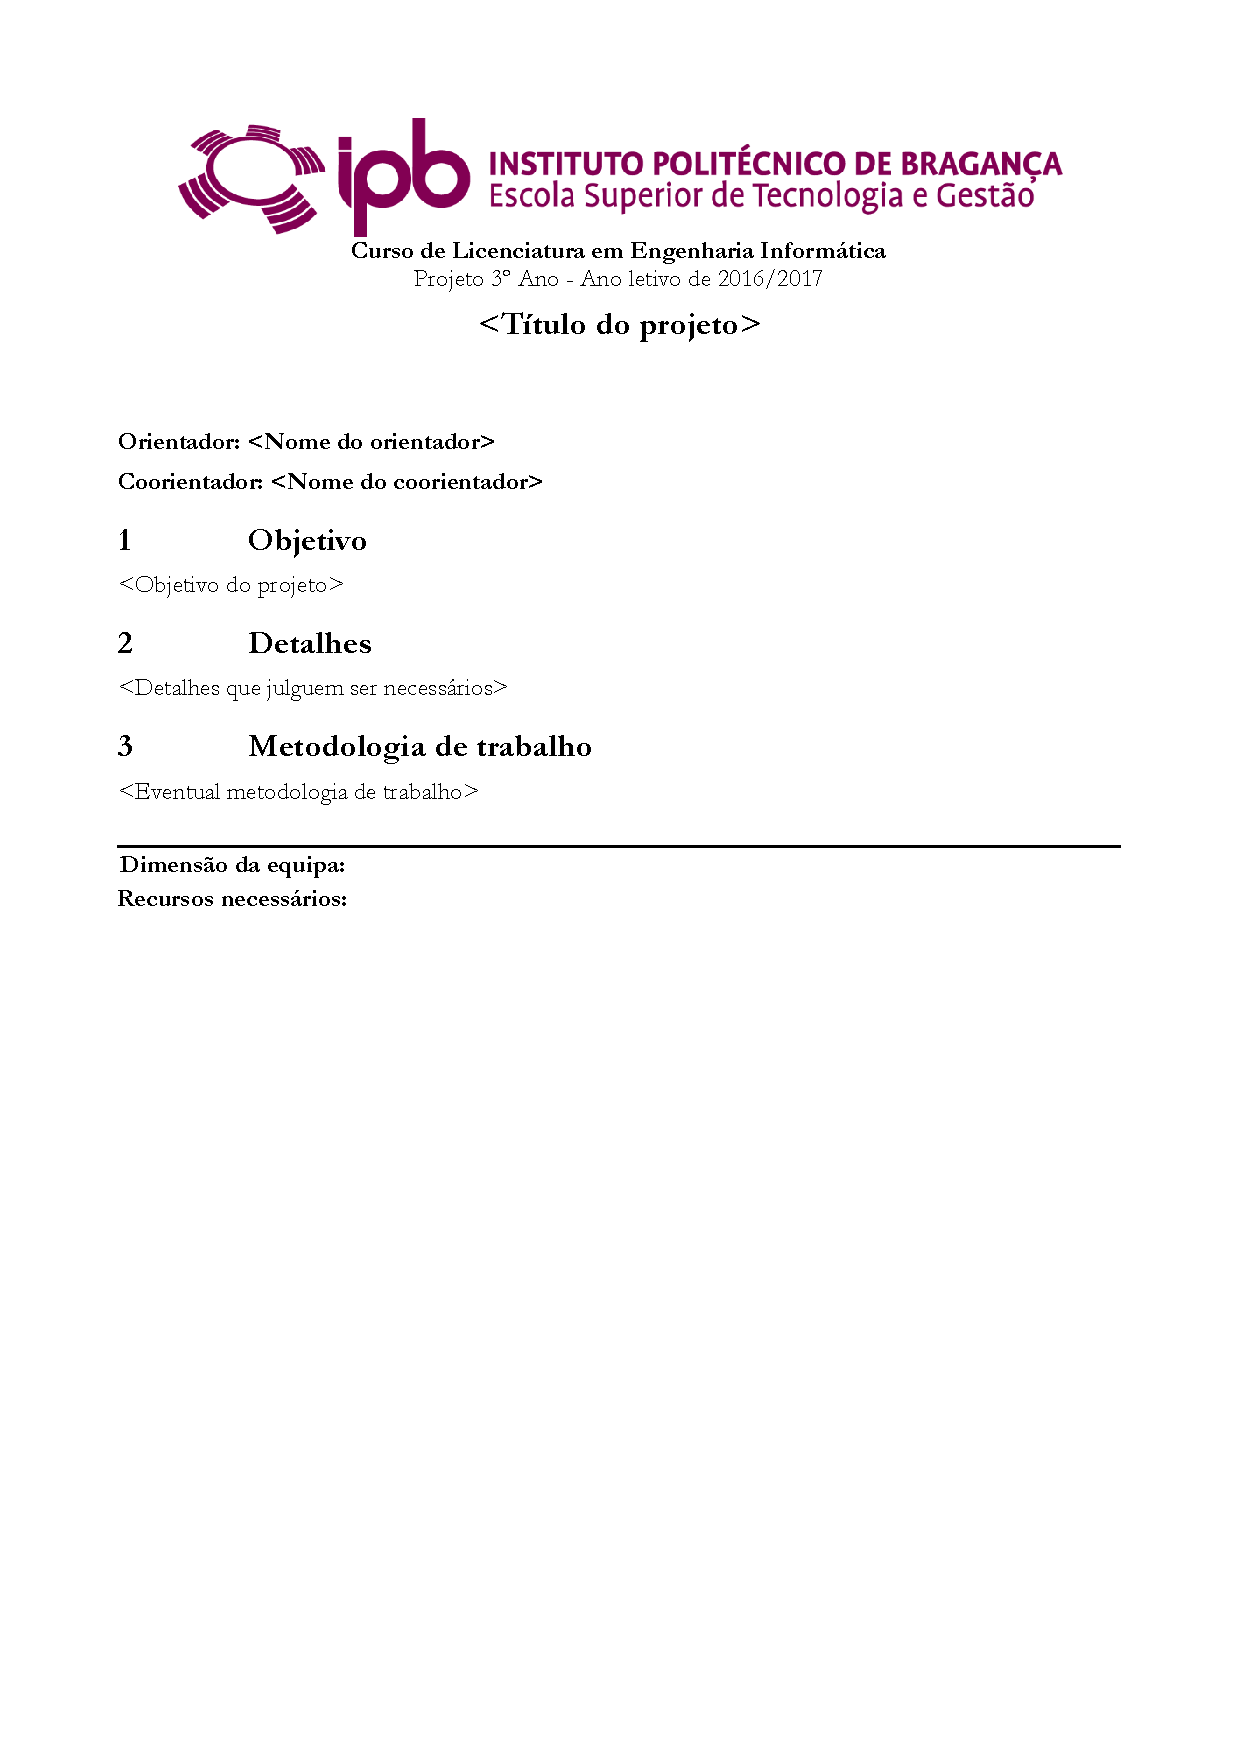
\includegraphics{etc/PropostaProjeto.pdf}
\end{figure}
%\chapter{Other appendix}
\label{apendice2}

Source code listing, text/images produces, complementary tests, etc.



\end{document}
